\documentclass[conference]{IEEEtran}
\IEEEoverridecommandlockouts
%Template version as of 6/27/2024

% Should probably be removed at some point!
\usepackage{silence}
\WarningsOff*

% \usepackage{xcolor}
\usepackage[table,usenames,dvipsnames]{xcolor}

\usepackage{amsmath,amssymb,amsfonts}
\usepackage{graphicx}

\usepackage{makecell, tabularx}
\renewcommand\theadalign{cc}
\renewcommand\theadfont{\bfseries}
\renewcommand\tabularxcolumn[1]{m{#1}}
\renewcommand{\arraystretch}{1.2}
\usepackage{pdflscape}
\usepackage{tablefootnote}

\usepackage{nameref}

% General Assets
%------------------------------------------------------------------------------
% Code
%------------------------------------------------------------------------------

\input{assets/code/names}
\input{assets/misc/posterHelpers}

% for assets/code/example.tex...
\newcommand{\exampleCode}{\input{assets/code/example}}
\newcommand{\refExampleCode}{\Cref{lst:exampleCode}}

% for assets/code/examplePseudocode.tex...
\newcommand{\examplePseudocode}{\input{assets/code/examplePseudocode}}
\newcommand{\refExamplePseudocode}{\Cref{lst:examplePseudocode}}

% for assets/code/mainInvalidInputTest.tex...
\newcommand{\mainInvalidInputTest}{\input{assets/code/mainInvalidInputTest}}
\newcommand{\refMainInvalidInputTest}{\Cref{lst:mainInvalidInputTest}}

% for assets/code/projManualViolationReq.tex...
\newcommand{\projManualViolationReq}{\input{assets/code/projManualViolationReq}}
\newcommand{\refProjManualViolationReq}{\Cref{lst:projManualViolationReq}}

% for assets/code/projViolationChoice.tex...
\newcommand{\projViolationChoice}{\input{assets/code/projViolationChoice}}
\newcommand{\refProjViolationChoice}{\Cref{lst:projViolationChoice}}

%------------------------------------------------------------------------------
% Graphs
%------------------------------------------------------------------------------

% Organization of files

% \newcommand{\parChdGraphs}{
%     % Only top or bottom to comply with IEEE guidelines
%     \begin{figure}[tb!]
%         \centering
%         \begin{subfigure}[b]{\linewidth}
%             \centering
%             \includegraphics[width=\linewidth]{assets/graphs/specBasedGraph.pdf}
%             \caption{``Superset'' relations.}
%             \label{fig:specBasedGraph}
%         \end{subfigure}
%         \begin{subfigure}[t]{.45\linewidth}
%             \centering
%             \includegraphics[width=\linewidth]{assets/graphs/parChdLegend.pdf}
%         \end{subfigure}
%         \begin{subfigure}[t]{.5\linewidth}
%             \centering
%             \includegraphics[width=\linewidth]{assets/graphs/subsumesGraph.pdf}
%             \caption{``Subsume'' relations.}
%             \label{fig:subsumesGraph}
%         \end{subfigure}
%         \caption{Visualizations of different classes of parent-child relations.}
%         \label{fig:parChdGraphs}
%     \end{figure}
% }

\newcommand{\ExampleParChdGraphs}{
    % Only top or bottom to comply with IEEE guidelines
    \begin{figure*}[tb!]
        \begin{subfigure}[b]{0.4\linewidth}
            \includegraphics[width=0.9\linewidth]{assets/graphs/ExampleGlossaryGraph.pdf}
            \vspace{-8mm}
            \caption{Visualization from \\ \Cref{tab:exampleGlossary}.}
            \label{fig:exampleGraph}
        \end{subfigure}
        \centering
        \begin{subfigure}[b]{0.575\linewidth}
            \centering
            \includegraphics[width=\linewidth]{assets/graphs/manual/manualParChdLegend.pdf}
            % \vspace{-4mm}  % Not working for some reason
            \includegraphics[width=0.8\linewidth]{assets/graphs/expExampleGlossaryGraph.pdf}
            \vspace{-8mm}
            \caption{Explicit visualization from \\ \Cref{tab:exampleGlossary}.}
            \label{fig:expExampleGraph}
        \end{subfigure}
        \vspace{2mm}
        \caption{Example generated visualizations of parent-child relations.}
        \label{fig:exampleParChdGraphs}
    \end{figure*}
}

\newcommand{\ExampleSynGraph}{
    \begin{figure*}
        \begin{subfigure}[c]{0.4\linewidth}
            \centering
            \includegraphics[width=\linewidth]{assets/graphs/SynExampleGlossaryGraph.pdf}
            \caption{Visualization from \Cref{tab:synExampleGlossary}.} %\label{fig:exampleSynGraph}
        \end{subfigure}
        \begin{subfigure}[c]{0.575\linewidth}
            \centering
            \includegraphics[width=\linewidth]{assets/graphs/manual/manualSynLegend.pdf}
        \end{subfigure}
        \caption{Example generated visualizations of synonym relations.}\label{fig:exampleSynGraph}
    \end{figure*}
}

% \begin{subfigure}[t]{0.25\linewidth}
%     \centering
%     \includegraphics[width=1.4\linewidth]{assets/graphs/StaticExampleGlossaryGraph.pdf}
%     \caption{Static graph.}
%     \label{fig:staticExampleGraph}
% \end{subfigure}

\newcommand{\ExampleFlawGraphs}{
    \begin{figure*}
        \begin{subfigure}[t]{0.19\linewidth}
            \centering
            \includegraphics[width=1.5\linewidth]{assets/graphs/SelfExampleGlossaryGraph.pdf}
            \caption{Visualization of a reflexive parent relation.}\label{fig:selfExampleGraph}
        \end{subfigure}
        \hfill
        \begin{subfigure}[t]{0.235\linewidth}
            \centering
            \includegraphics[width=\linewidth]{assets/graphs/ParSynExampleGlossaryGraph.pdf}
            \caption{Visualization of a pair of terms with a parent-child \emph{and}
                synonym relation.}\label{fig:parSynExampleGraph}
        \end{subfigure}
        \hfill
        \begin{subfigure}[t]{0.47\linewidth}
            \centering
            \includegraphics[width=\linewidth]{assets/graphs/manual/manualFlawLegend.pdf}
        \end{subfigure}
        \caption{Example generated visualizations containing flaws.}\label{fig:exampleFlawGraphs}
    \end{figure*}
}

\newcommand{\recoveryGraphs}{
    % Only top or bottom to comply with IEEE guidelines
    \begin{figure}[bt!]
        \centering
        \includegraphics[width=\linewidth]{assets/graphs/recoveryLegend.pdf}
        \begin{subfigure}[b]{.475\linewidth}
            \centering
            \includegraphics[width=\linewidth]{assets/graphs/recoveryGraph.pdf}
            \caption{Visualization of current relations.}
            \label{fig:rec-graph-current}
        \end{subfigure}
        \begin{subfigure}[b]{.475\linewidth}
            \centering
            \includegraphics[width=\linewidth]{assets/graphs/recoveryProposedGraph.pdf}
            \caption{Visualization of proposed relations.}
            \label{fig:rec-graph-proposed}
        \end{subfigure}
        \caption{Visualizations of relations between terms related to recovery testing.}
        \label{fig:recoveryGraphs}
    \end{figure}
}

\newcommand{\scalGraphs}{
    % Only top or bottom to comply with IEEE guidelines
    \begin{figure}[b!]
        \centering
        \includegraphics[width=\linewidth]{assets/graphs/scalabilityLegend.pdf}
        \begin{subfigure}[b]{.475\linewidth}
            \centering
            \includegraphics[width=\linewidth]{assets/graphs/scalabilityGraph.pdf}
            \caption{Visualization of current relations.}
            \label{fig:scal-graph-current}
        \end{subfigure}
        \begin{subfigure}[b]{.475\linewidth}
            \centering
            \includegraphics[width=\linewidth]{assets/graphs/scalabilityProposedGraph.pdf}
            \caption{Visualization of proposed \ifnotpaper \else \\ \fi relations.}
            \label{fig:scal-graph-proposed}
        \end{subfigure}
        \caption{Visualizations of relations between terms related to scalability testing.}
        \label{fig:scalGraphs}
    \end{figure}
}

\newcommand{\performanceGraph}{
    \begin{paperFigure}
        \centering
        \includegraphics[width=\linewidth]{assets/graphs/performanceProposedGraph.pdf}
        \caption{Visualization of proposed relations between terms related to
            performance-related testing.}
        \label{fig:perf-graph}
    \end{paperFigure}
}

%------------------------------------------------------------------------------
% Images & Figures
%------------------------------------------------------------------------------

\newcommand{\drasilLogo}{assets/images/drasil_logo.png}
\newcommand{\drasilLogoImg}{\input{assets/images/drasil_logo}}
\newcommand{\refDrasilLogoImg}{\Cref{fig:drasilLogo}}

%------------------------------------------------------------------------------
% Tables
%------------------------------------------------------------------------------

% Organization of files
\newcommand{\organizationTable}{\input{assets/tables/organization}}

\newcommand{\ieeeCatsTable}{\input{assets/tables/ieeeCats}}
\newcommand{\otherCatsTable}{\input{assets/tables/otherCats}}
\newcommand{\otherCategorizationsTable}{\input{assets/tables/otherCategorizations}}

\newcommand{\flawMnfstsTable}{\input{assets/tables/flawMnfsts}}
\newcommand{\flawDmnsTable}{\input{assets/tables/flawDmns}}

\newcommand{\testReqsTable}{\input{assets/tables/testReqs}}


% Enable links within the document
\usepackage{hyperref}
\hypersetup{
    colorlinks=true,
    linkcolor=red,
    urlcolor=red,
    breaklinks=true
}
\urlstyle{rm} % Make URL styled fonts match hyperref's hrefs
\usepackage{cleveref} % Fixes capitalization of internal references

% General Utility Functions
%------------------------------------------------------------------------------
% Spacing Options
%------------------------------------------------------------------------------

\newcommand{\thesisForceSingleSpacing}{\singlespacing}
\newcommand{\thesisForceDoubleSpacing}{\doublespacing}

%------------------------------------------------------------------------------
% Portable HREFs
%------------------------------------------------------------------------------

% Common variant
\newcommand{\porthref}[2]{\href{#2}{#1}\printOnlyFootnote{\url{#2}}}

% Custom URLs
\newcommand{\porthreft}[3]{\href{#3}{#1}\printOnlyFootnote{\href{#3}{#2}}}
% Inside of some environments, footnote marks aren't registered properly, so we
% need to manually write the "text" part
\newcommand{\porthreftm}[2]{\href{#2}{#1\printOnlyFootnoteMark}}

%------------------------------------------------------------------------------
% Optional namerefs in context of (see <section name>)
%------------------------------------------------------------------------------

\newif\ifusenamerefs
\newcommand{\seeSection}[1]{%
  \ifusenamerefs
    { see \nameref{#1}}%
  \fi
}
\newcommand{\seeSectionPar}[2]{%
  \ifusenamerefs
    { (see \nameref{#1}#2)}%
  \fi
}
\newcommand{\seeSectionFoot}[1]{%
  \ifusenamerefs
    {\footnote{See \nameref{#1}.}}%
  \fi
}

%------------------------------------------------------------------------------
% TODOs
%------------------------------------------------------------------------------

% Generic Inlined TODOs
\newcommand{\intodo}[1]{\todo[inline]{#1}}

% Unimportant TODOs for "later" (i.e., finishing touches or changes immediately before submission)
\newcommand{\latertodo}[1]{\todo[backgroundcolor=Cyan]{\textit{Later}: #1}}

% "Important" TODOs
\newcommand{\imptodo}[1]{\todo[inline,backgroundcolor=Red]{\textbf{Important}: #1}}

% "Easy" TODOs
\newcommand{\easytodo}[1]{\todo[inline,backgroundcolor=SeaGreen]{\textit{Easy}: #1}}
\newcommand{\eztodo}[1]{\easytodo{#1}}

% "Tedious" TODOs
\newcommand{\tedioustodo}[1]{\todo[inline,backgroundcolor=PineGreen]{\textit{Needs time}: #1}}

% "Question" TODO Notes
\newcounter{todonoteQuestionsCtr}
\newcommand{\questiontodo}[1]{\stepcounter{todonoteQuestionsCtr}\todo[backgroundcolor=Lavender]{\textbf{Q \#\thetodonoteQuestionsCtr{}}: #1}}
\newcommand{\qtodo}[1]{\questiontodo{#1}}

%------------------------------------------------------------------------------
% Citations
%------------------------------------------------------------------------------

\newcommand{\exhInfCite}{(\citealp[p.~5-5]{SWEBOK2024}; \citealp[p.~4]{IEEE2022};
  \citealp[p.~421]{vanVliet2000}; \citealp[pp.~439, 461]{PetersAndPedrycz2000})}

%------------------------------------------------------------------------------
% Link to Drasil issue
%------------------------------------------------------------------------------

\newcommand{\issueref}[1]{\href{https://github.com/JacquesCarette/Drasil/issues/#1}{\##1}}
\newcommand{\pullref}[1]{\href{https://github.com/JacquesCarette/Drasil/pull/#1}{\##1}}
\newcommand{\thesisissueref}[1]{\href{https://github.com/samm82/TestGen-Thesis/issues/#1}{\##1}}



\usepackage{cite}
\newcommand{\citetISTQB}{\cite{ISTQB}}
\newcommand{\citepISTQB}{\cite{ISTQB}}
\newcommand{\citealpISTQB}{\cite{ISTQB}}
\newcommand{\citeauthor}{\cite}
\newcommand{\citeauthorpar}{\cite}
\newcommand{\citeyearpar}{\cite}
\newcommand{\citeyear}{\cite}
\newcommand{\citet}{\cite}
\newcommand{\citep}{\cite}
\newcommand{\citealp}{\cite}
\newcommand{\citetext}[1]{[#1]}

\usepackage{algorithmic}
\usepackage{textcomp}

\usepackage[disable]{todonotes}

\newenvironment{paperTable}{
    \begin{table*}[t]
        }{
    \end{table*}
}

\newenvironment{paperFigure}{
    \begin{figure*}[t]
        }{
    \end{figure*}
}

\def\BibTeX{{\rm B\kern-.05em{\sc i\kern-.025em b}\kern-.08em
    T\kern-.1667em\lower.7ex\hbox{E}\kern-.125emX}}
\begin{document}

\title{\paperTitle{}\\
    % Sub-titles should not be used!
    \ifblind{\thanks{Funding information suppressed.\vspace{4mm}}}
    {\thanks{Funding for this work was provided by the Ontario Graduate
            Scholarship and McMaster University.}
    }
}

\author{
    \ifblind{Author details suppressed\vspace{18mm}}
    {\IEEEauthorblockN{Samuel J. Crawford\IEEEauthorrefmark{1},
            Spencer Smith\IEEEauthorrefmark{1}, Jacques Carette\IEEEauthorrefmark{1}}
        \IEEEauthorblockA{\IEEEauthorrefmark{1}Department of Computing and Software \\
            McMaster University\\
            Hamilton, Canada \\
            \{crawfs1, smiths, carette\}@mcmaster.ca}}}

% % Previous version (weird formatting)
% \newcommand{\deptCAS}[1]{
%     \IEEEauthorblockA{\textit{Department of Computing and Software} \\
%         \textit{McMaster University}\\
%         Hamilton, Canada \\
%         #1@mcmaster.ca}}

% \author{\IEEEauthorblockN{Samuel~J.~Crawford}
%     \deptCAS{crawfs1}
%     \and
%     \IEEEauthorblockN{Spencer~Smith}
%     \deptCAS{smiths}
%     \and
%     \IEEEauthorblockN{Jacques~Carette}
%     \deptCAS{carette}
% }

\maketitle

\begin{abstract}
    Testing is a pervasive software development activity that is often
    complicated and expensive (if not simply overlooked), partly due to
    the lack of a standardized and consistent taxonomy for software testing.
    This hinders precise communication, leading to discrepancies and
    ambiguities across the literature and even within individual documents!
    % Therefore, automating the software testing process is an area of interest,
    % and understanding the underlying domain is an important prerequisite.
    In this paper, we systematically examine the current state of software
    testing terminology. We 1) identify established standards
    and prominent testing resources, 2) capture relevant testing terms
    from these sources, along with their definitions and relationships---both
    explicit and implied---and 3) construct graphs to visualize and analyze
    this data. Our research uncovered more than 500 test approaches and
    four methods for describing ``implied'' test approaches. We also build
    a tool for generating graphs that illustrate relations between test
    approaches and track ambiguities captured by this tool and manually through
    the research process. Our results reveal \ref*{totalDiscreps} discrepancies
    or ambiguities, including ten terms used as synonyms to two (or more)
    disjoint test approaches and \parSynAll{} pairs of test approaches may
    either be synonyms or have a child-parent relationship. Confusion was notable
    around functional, recovery, scalability, and performance testing,
    along with 45 other discrepancies. These findings make clear the urgent
    need for improved testing terminology so that the discussion, analysis and
    implementation of various test approaches can be more coherent. We
    provide some preliminary advice on how to achieve this standardization.
\end{abstract}

\begin{IEEEkeywords}
    Software testing, terminology, taxonomy, literature review, test approaches
\end{IEEEkeywords}

\section{Background}

% TODO: tighten up, add sources

Testing software is complicated, expensive, and often overlooked.
Improving the productivity of testing and testing research requires a standard
language for communication. Unfortunately, a search
for a systematic, rigorous, and ``complete'' taxonomy for software testing
revealed that the existing ones are inadequate:

\begin{itemize}
    \item \ifnotpaper\else Tebes et al. \fi\citet{TebesEtAl2020a} focus on
          \emph{parts} of the testing process (e.g., test goal, testable entity),
    \item \ifnotpaper\else Souza et al. \fi\citet{SouzaEtAl2017} prioritize
          organizing testing approaches over defining them, and
    \item \ifnotpaper\else Unterkalmsteiner et al. \fi\citet{UnterkalmsteinerEtAl2014}
          provide a foundation for classification but not how it applies to software
          testing terminology.
\end{itemize}

Thus we set about closing this gap. We first define the scope of what kinds of
``software testing'' are of interest (\Cref{scope}) and examine the existing
literature (\Cref{methodology}). This reinforces the need for a proper taxonomy!
Despite the amount of well understood and organized knowledge (\Cref{observ}),
there are still many discrepancies and ambiguities in the literature, either
within the same source or between various sources (\Cref{discrep}). We provide
some potential solutions covering some of these discrepancies (\Cref{recs}).
\section{Scope}
\label{scope}

Since our motivation is restricted to testing code, only this component of
\acf{vnv} is considered\thesisissueref{22}. However, some test approaches
are used for testing things other than code, and some approaches can be used
for both! In these cases, only the subsections of these approaches focused on
code are considered. For example, reliability testing and maintainability
testing can start \emph{without} code by ``measur[ing] structural attributes
of representations of the software'' \citep[p.~18]{FentonAndPfleeger1997}, but
only reliability and maintainability testing performed on code \emph{itself} is
in scope of this research.
\ifnotpaper
    In this section, we provide a high-level overview of what is in scope. We
    exclude some practices either in full, such as hardware testing
    (\Cref{hard-test}), or in part, such as parts of error seeding, fault
    injection testing, and mutation testing that do not directly test code
    (\Cref{other-vnv}).
    % More specific refs are used for now, since the following label points to
    %   Section 9.4 instead of Appendix A for some reason
    % (see \Cref{app-scope} for more detailed discussion on what we exclude).
    Additionally, static testing is a useful component of software testing and
    is therefore included at this level of analysis, despite it not being
    relevant to our original motivation (\Cref{static-test}). Finally, some
    test approaches can be derived from other categories of testing-related
    terminology (\Cref{derived-tests}); of these, approaches derived from
    programming languages (\Cref{lang-test}) or other orthogonal test
    approaches (\Cref{orth-test}) are out of scope.
\fi
\section{Methodology}
\label{methodology}

At a high level\todo{Is this sufficient as a chapter ``roadmap'', or should I
    include one explicitly? How would I do this without duplication?}, our
methodology follows the following steps:

\input{build/methodOverview}

\def\addTextEx{For example, \citetISTQB{} \multiAuthHelper{cite}
    \citep{GerrardAndThompson2002} as the original source
    for \ifnotpaper their \else its \fi definition of ``scalability'' (see
    \Cref{scal-test-rec}); we verified\ptq{} this by
    looking at this original source.}

\subsection{Sources}
\label{sources}
As there is no single authoritative source on software testing terminology,
we need to look at many to see how various terms are used in practice.
Starting from some widely used\todo{Justified in their respective sections;
    should I put pointers here?} sources (some IEEE standards and the
\acf{swebok}, \suggSrcs{}), we then use a version of ``snowball sampling'' to
gather further sources. Snowball sampling ``is commonly used to locate hidden
populations \dots{} [via] referrals from initially sampled respondents to other
persons'' \citep{Johnson2014}. We apply this concept to ``referrals'' between
sources. \addTextEx{} We also ``snowball'' on terminology itself in a similar
manner; when a term arises that requires more investigation (e.g., it is
undefined or unclear), a miniature literature review is performed in this
subset to ``fill in'' this missing information (see \Cref{undef-terms}). These
additional sources may then be investigated in their entirety (as opposed to
just the original subset of interest) if they provide more information and are
``trustworthy'', where more trustworthy sources:
\begin{enumerate}
    \item have gone through a peer-review process,
    \item are written by numerous, well-respected authors,
    \item are informed by many sources, and
    \item are accepted and used in the field of software.
\end{enumerate}

For ease of discussion and analysis, the complete set of sources can be grouped
based on their format, method of publication, and this metric of
``trustworthiness''. We therefore create the following tiers, given in order of
descending trustworthiness: established standards (\Cref{stds}), terminology
collections (\Cref{metas}), textbooks (\Cref{texts}), and papers and other
documents (\Cref{papers}). Note that most sources used to ``fill in'' missing
information are papers. A summary of how many sources comprise each tier is
given in \Cref{fig:sourceSummary}.

% Only top or bottom to comply with IEEE guidelines
\begin{figure}[bt!]
    \centering
    \begin{tikzpicture}
        \pie[sum=auto, after number=, text=legend, thick,
            scale=\ifnotpaper0.7\else0.5\fi,
            every label/.style={align=left, scale=0.7}]
        {\stdSources{3}/\stds{},
            \metaSources{3}/\metas{},
            \textSources{3}/\texts{},
            \paperSources{3}/\papers{}}
    \end{tikzpicture}
    \caption{Summary of how many sources comprise each source tier.}
    \label{fig:sourceSummary}
\end{figure}

\ifnotpaper\newpage\fi

\subsubsection{\stdSources{1}}
\label{stds}
% Colored \textcolor{green}{green}

These are documents written for the field of software engineering by reputable
standards bodies, namely ISO, the \acf{iec}, and IEEE. We only consider those
about software development and testing for the purposes of this research (see
\Cref{scope}). For example, ``the purpose of the ISO/IEC/IEEE 29119 series is
to define an internationally agreed set of standards for software testing that
can be used by any organization when performing any form of software testing''
\ifnotpaper(\fi\citealp[p.~vii]{IEEE2022}\ifnotpaper; similar in
\citeyear[p.~ix]{IEEE2016})\fi. This tier is composed of \stdSources{2}.

\subsubsection{\metaSources{1}}
\label{metas}
% Colored \textcolor{blue}{blue}

These are collections of software testing terminology built up from multiple
sources, including established standards (see \Cref{stds}). These documents are
made to be widely applicable; for example, the \acs{swebok} is ``proposed as a
suitable foundation for government licensing, for the regulation of software
engineers, and for the development of university curricula in software
engineering'' \citep[p.~xix]{KanerEtAl2011}. They are often written by a large
organization, such as the \acf{istqb}, but not always. We include
\citeauthor{Firesmith2015}'s taxonomy \citeyearpar{Firesmith2015} because it
presents relations between many test approaches and \citeauthor{DoğanEtAl2014}'s
literature review \citeyearpar{DoğanEtAl2014} because it cites a large number
of sources from which we can ``snowball'' if desired (see \Cref{sources}).
This tier is composed of \metaSources{2}.

\subsubsection{\textSources{1}}
\label{texts}
% Colored \textcolor{Maroon}{maroon}

We consider textbooks to be more trustworthy than papers (see \Cref{papers})
because they are widely used as resources for teaching software engineering and
may be used as guides in industry. Although textbooks have smaller sets of
authors, they follow a formal review process before publication. Textbooks that
are trusted at McMaster \citep{Patton2006, PetersAndPedrycz2000, vanVliet2000}
served as the original (albeit ad hoc and arbitrary) starting point of this
research; we investigate other books as they arise. \addTextEx{}
This tier is composed of \textSources{2}.

\subsubsection{\paperSources{1}}
\label{papers}
% Colored black

Documents in this source tier are written by much smaller sets of authors
% with unknown peer review processes % TODO: investigate
and are much less widespread than higher source tiers.
While most documents are journal articles and conference papers, the following
document types are also present; some less-than-academic sources show how terms
are used in practice and are included in this source tier for brevity%
\thesisissueref{89}:

\begin{itemize}
    \item Report \citep{Kam2008,Gerrard2000a,Gerrard2000b}
    \item Thesis \citep{Bas2024}
          % \item A less-formal classification \citep{KuļešovsEtAl2013}
    \item Website \citep{LambdaTest2024,Pandey2023}
    \item Booklet \citep{SPICE2022}
    \item \ifnotpaper \else ChatGPT \fi \citet{ChatGPT2024} (with its claims
          supported by \citet{RusEtAl2008})
\end{itemize}

The full set of sources that comprise this tier is \paperSources{2}.

% Moved here to display nicely in paper
\ifnotpaper\else
    % Only top or bottom to comply with IEEE guidelines
    \begin{table*}[t!]
        %     \begin{minipage}{\linewidth}
        \ieeeCatsTable{}
        %     \end{minipage}
    \end{table*}
\fi

\subsection{Terminology}

\def\rigidBlurb{While most information is presented explicitly in the sources
    we investigate, some appears more implicitly. This is a useful distinction
    to make, as implicit claims carry less weight than explicit ones. We call
    this property ``rigidity''}

This research is intended to describe the current state of software testing
literature. To reduce potential bias, we do not invent or add our own
classifications or kinds of relations. Instead, the notions of test approach
categories (\Cref{categories-observ}), synonyms (\Cref{syn-rels}), and
parent-child relations (\Cref{par-chd-rels}) presented here
arose\ptq{} naturally from the literature. We define them here for clarity
since we use them throughout this \ifnotpaper thesis\else paper\fi, even
though they are ``results'' of our research. \rigidBlurb{} and define it
in \Cref{rigidity}.

\subsubsection{Approach Categories}
\label{categories-observ}

While there are many ways to categorize software testing approaches, perhaps
the most widely used is the one given by \ifnotpaper\else \citeauthor{IEEE2022}
\fi \citet{IEEE2022}, where a test approach can be categorized as a test level,
test type, test technique, or test practice (see \Cref{tab:ieeeCats}).
The categories of ``level'' and ``type'' are particularly common; for example,
six non-IEEE sources also give unit testing, integration testing,
system testing, and acceptance testing as examples of test levels \ifnotpaper
    (\citealp[pp.~5\=/6 to 5\=/7]{SWEBOK2024}; \citealpISTQB{};
    \citealp[pp.~807--808]{Perry2006}; \citealp[pp.~443--445]{PetersAndPedrycz2000};
    \citealp[p.~218]{KuļešovsEtAl2013}\todo{OG Black, 2009};
    \citealp[pp.~9, 13]{Gerrard2000a})\else
    \cite[pp.~443--445]{PetersAndPedrycz2000}, \cite{ISTQB},
    \cite[pp.~5\=/6 to 5\=/7]{SWEBOK2024}, \cite[pp.~9, 13]{Gerrard2000a},
    \cite[pp.~807--808]{Perry2006}, \cite[p.~218]{KuļešovsEtAl2013}%
    \todo{OG Black, 2009}\fi, although they may use a different term for ``test
level'' (see \Cref{tab:ieeeCats}). Because of their widespread use and
their usefulness in dividing the domain of software testing into more
manageable subsets, these categories are used for now. These four subcategories
of test approaches can be loosely described by what they specify as
follows\thesisissueref{21}:
\begin{itemize}
    \item \textbf{Level}: What code is tested
    \item \textbf{Practice}: How the test is structured and executed
    \item \textbf{Technique}: How to derive inputs and/or outputs
    \item \textbf{Type}: Which software quality is evaluated
\end{itemize}
For example, boundary value analysis is a test technique since its inputs are
``the boundaries of equivalence partitions'' \ifnotpaper
    (\citealp[p.~2]{IEEE2022}; \citeyear[p.~1]{IEEE2021}; similar on p.~12 and
    in \citealpISTQB{})%
\else
    \cite[p.~2]{IEEE2022}, \cite[p.~1]{IEEE2021}%
\fi. Similarly, acceptance testing is a test level since its goal is to
``enable a user, customer, or other authorized entity to determine whether to
accept a system or component'' \ifnotpaper (\citealp[p.~5]{IEEE2017}; similar
    in \citeyear[p.~6]{IEEE2021}; \citealp[p.~344]{SakamotoEtAl2013})\else
    \cite[p.~5]{IEEE2017}\fi, which requires the system or component to be
developed and ready for testing.

While the vast majority of identified test approaches can be categorized
in this way, \ifnotpaper there seem to be some outliers. For example, \fi
we also note the potential significance of an ``artifact'' category%
\thesisissueref{44,119,39}, since some terms could refer to the application of
a test approach and/or the resulting document(s). Because of this, a test
approach being categorized as a category from \Cref{tab:ieeeCats}
\emph{and} an artifact is \emph{not} a discrepancy\thesisissueref{119}
(see \Cref{multiCats}). \ifnotpaper
    Additionally, ``test metrics'' were also identified\thesisissueref{21,22},
    but tracking them is out-of-scope, since they describe methods for
    \emph{evaluating} testing as opposed to methods for \emph{performing} it.
    The related test approaches that seek to maximize these metrics are instead
    captured as kinds of coverage-driven testing (see \Cref{cov-test}) and
    experience-based testing \citep[p.~34]{IEEE2022}. \par \fi
Excluding \ifnotpaper our proposed \else this \fi ``artifact'' category, the
categories given in \Cref{tab:ieeeCats} seem to be orthogonal. For
example, ``a test type can be performed at a single test level or across
several test levels''
\ifnotpaper
    (\citealp[p.~15]{IEEE2022}; \citeyear[p.~7]{IEEE2021})%
\else
    \cite[p.~15]{IEEE2022}, \cite[p.~7]{IEEE2021}%
\fi, and ``Keyword-Driven Testing [sic] can be applied at all testing levels
(e.g. [sic] component testing, system testing) and for various types of testing
(e.g. [sic] functional testing\footnote{See \Cref{corr-func-test}.}, reliability
testing)'' \citeyearpar[p.~4]{IEEE2016}. This means that a specific test
approach can be derived by combining multiple test approaches from different
categories; for example, formal reviews are a combination of formal testing and
reviews. \ifnotpaper The following examples
    are given in the literature; the two subapproaches for each are omitted
    for brevity as the name of the combination makes it clear what they are:

    \phantomsection{}\label{orth-test-exs}
    \begin{enumerate}
        \item Black box conformance testing \citep[p.~25]{JardEtAl1999}
              %   (combining black box and conformance testing)
              % Specification-based: Technique (IEEE, 2022, p. 22; 2021, p. 8; Washizaki, 2024, p. 5-10; Hamburg and Mogyorodi, 2024; Souza et al., 2017, p. 3; Firesmith, 2015, pp. 46-47; Sakamoto et al., 2013, p. 344; implied by IEEE, 2022, pp. 2-4, 6-9)
              % Conformance: Type (implied by its quality (IEEE, 2017, p. 92; OG PMBOK 5th ed.))
        \item Black-box integration testing \citep[pp.~345--346]{SakamotoEtAl2013}
              % Specification-based: Technique (IEEE, 2022, p. 22; 2021, p. 8; Washizaki, 2024, p. 5-10; Hamburg and Mogyorodi, 2024; Souza et al., 2017, p. 3; Firesmith, 2015, pp. 46-47; Sakamoto et al., 2013, p. 344; implied by IEEE, 2022, pp. 2-4, 6-9)
              % Integration: Level (IEEE, 2022, pp. 12, 20-22, 26-27; 2021, p. 6; Washizaki, 2024, p. 5-7; Hamburg and Mogyorodi, 2024; Sakamoto et al., 2013, p. 343; Peters and Pedrycz, 2000, Tab. 12.3; van Vliet, 2000, p. 438; implied by Barbosa et al., 2006, p. 3)
              %           OR Technique (implied by Sharma et al., 2021, pp. 601, 603, 605-606)
        \item Checklist-based reviews \citepISTQB{}
              % Checklist-based: Practice (IEEE, 2022, p. 34), Technique (Hamburg and Mogyorodi, 2024)
              % Reviews: Approach
        \item Closed-loop HiL verification \citep[p.~6]{PreußeEtAl2012}
              % Closed Loop: Technique?
              % HiL: Out of Scope (hardware)
        \item Closed-loop protection system testing \citep[p.~331]{ForsythEtAl2004}
              % Closed Loop: Technique?
              % System: Level (IEEE, 2022, pp. 12, 20-22, 26-27; 2021, p. 6; 2017, p. 467; 2016, p. 4; Washizaki, 2024, p. 5-7; Hamburg and Mogyorodi, 2024; Sakamoto et al., 2013, p. 343; Peters and Pedrycz, 2000, Tab. 12.3; van Vliet, 2000, p. 439; implied by Barbosa et al., 2006, p. 3; Gerrard, 2000a, p. 13)
        \item Endurance stability testing \citep[p.~55]{Firesmith2015}
              % Endurance: Type (IEEE, 2013, p. 2; implied by Firesmith, 2015, p. 55)
              %         OR Technique (IEEE, 2021, p. 38)
              % Stability: Type (implied by its quality (IEEE, 2017, p. 434; OG ISO/IEC, 2009) and Firesmith, 2015, p. 55)
        \item End-to-end functionality testing (\citealp[p.~20]{IEEE2021}; \citealp[Tab.~2]{Gerrard2000a})
              % End-to-end: Type (Hamburg and Mogyorodi, 2024)
              %          OR Technique (Firesmith, 2015, p. 47; Sharma et al., 2021, pp. 601, 603, 605-606)
              % Functionality: Type (implied by its quality (IEEE, 2017, p. 196); Firesmith, 2015, p. 53)
        \item Formal reviews \citepISTQB{}
              % Formal: Technique (inferred from informal testing)
              % Reviews: Approach
        \item Grey-box integration testing \citep[p.~344]{SakamotoEtAl2013}
              % Grey-Box: Technique (IEEE, 2021, p. 8; Firesmith, 2015, pp. 46, 48; Sakamoto et al., 2013, p. 344)
              % Integration: Level (IEEE, 2022, pp. 12, 20-22, 26-27; 2021, p. 6; Washizaki, 2024, p. 5-7; Hamburg and Mogyorodi, 2024; Sakamoto et al., 2013, p. 343; Peters and Pedrycz, 2000, Tab. 12.3; van Vliet, 2000, p. 438; implied by Barbosa et al., 2006, p. 3)
              %           OR Technique (implied by Sharma et al., 2021, pp. 601, 603, 605-606)
        \item Incremental integration testing \citep[p.~601, 603, 605--606]{SharmaEtAl2021}\todo{OG [19]}
              % Incremental: Practice?
              % Integration: Level (IEEE, 2022, pp. 12, 20-22, 26-27; 2021, p. 6; Washizaki, 2024, p. 5-7; Hamburg and Mogyorodi, 2024; Sakamoto et al., 2013, p. 343; Peters and Pedrycz, 2000, Tab. 12.3; van Vliet, 2000, p. 438; implied by Barbosa et al., 2006, p. 3)
              %           OR Technique (implied by Sharma et al., 2021, pp. 601, 603, 605-606)
        \item Informal reviews \citepISTQB{}
              % Informal: Technique (implied by Kam, 2008, p. 6)
              % Reviews: Approach
        \item Infrastructure compatibility testing \citep[p.~53]{Firesmith2015}
              % Infrastructure: Type (implied by Firesmith, 2015, p. 57)
              %              OR Level (implied by Gerrard, 2000a, p. 13; see \Cref{tab:ieeeCats})
              % Compatibility: Type (IEEE, 2022, pp. 3, 22; 2021, p. 37, Tab. A.1; 2013, p. 2; implied by its quality (ISO/IEC, 2023a); Firesmith, 2015, p. 53)
        \item Invariant-based automatic testing \citep[pp.~184--185, Tab.~21]{DoğanEtAl2014},
              including for ``AJAX user interfaces'' \citetext{p.~191}
              % Assertion Checking: Practice?
              % Automated: Practice (IEEE, 2022, pp. 20, 22)
              %         OR Technique (implied by p. 35)
        \item Legacy system integration (testing) \citep[Tab.~2]{Gerrard2000a}
              % Legacy: Approach
              % System Integration: Level (IEEE, 2022, pp. 12, 22; 2021, p. 6; Hamburg and Mogyorodi, 2024)
        \item Manual procedure testing \citep[p.~47]{Firesmith2015}
              % Manual: Practice (IEEE, 2022, p. 22)
              %      OR Technique (implied by p. 35)
              % Procedure: Type (IEEE, 2022, pp. 7, 22; 2021, p. 39, Tab. A.1; 2017, p. 337; OG IEEE, 2013)
              %         OR Technique (implied by Firesmith, 2015, p. 47)
        \item Manual security audits \citep[p.~28]{Gerrard2000b}
              % Manual: Practice (IEEE, 2022, p. 22)
              %      OR Technique (implied by p. 35)
              % Security Audits: Technique (IEEE, 2021, p. 40)
              %               OR Type (inferred from security testing)
        \item Model-based GUI testing (\citealp[Tab.~1]{DoğanEtAl2014}; implied by \citealp[p.~356]{SakamotoEtAl2013})
              % Model-based: Practice (IEEE, 2022, p. 22; 2021, p. viii)
              %           OR Technique (Engström and Petersen, 2015, pp. 1-2; Kam, 2008, p. 4; implied by IEEE, 2022, p. 32; 2021, p. 7; 2017, p. 469)
              % GUI: Approach
        \item Model-based web application testing (implied by \citealp[p.~356]{SakamotoEtAl2013})
              % Model-based: Practice (IEEE, 2022, p. 22; 2021, p. viii)
              %           OR Technique (Engström and Petersen, 2015, pp. 1-2; Kam, 2008, p. 4; implied by IEEE, 2022, p. 32; 2021, p. 7; 2017, p. 469)
              % Web Application: Approach
        \item Non-functional search-based testing \citep[Tab.~1]{DoğanEtAl2014}
              % Non-functional: Approach
              % Search-based: Technique (Engström and Petersen, 2015, pp. 1-2)
        \item Offline MBT \citepISTQB{}
              % Offline: Practice?
              % Model-based: Practice (IEEE, 2022, p. 22; 2021, p. viii)
              %           OR Technique (Engström and Petersen, 2015, pp. 1-2; Kam, 2008, p. 4; implied by IEEE, 2022, p. 32; 2021, p. 7; 2017, p. 469)
        \item Online MBT \citepISTQB{}
              % Online: Practice?
              % Model-based: Practice (IEEE, 2022, p. 22; 2021, p. viii)
              %           OR Technique (Engström and Petersen, 2015, pp. 1-2; Kam, 2008, p. 4; implied by IEEE, 2022, p. 32; 2021, p. 7; 2017, p. 469)
        \item Role-based reviews \citepISTQB{}
              % Role-based: Practice?
              % Reviews: Approach
        \item Scenario walkthroughs \citep[Fig.~4]{Gerrard2000a}
              % Scenario: Technique (IEEE, 2022, pp. 9, 22; 2021, pp. 5, 8, 20, Fig. 2; 2017, p. 400; OG 2013; Washizaki, 2024, p. 5-12; Firesmith, 2015, p. 47; Sangwan and LaPlante, 2006, p. 26)
              % Walkthroughs: Technique (IEEE, 2017, p. 508)
        \item Scenario-based reviews \citepISTQB{}
              % Scenario-based: Approach
              % Reviews: Approach
        \item Security attacks \citepISTQB{}
              % Security: Type (IEEE, 2022, pp. 9, 22, 26-27; 2021, pp. 7, 40, Tab. A.1; 2017, p. 405; OG 2013; implied by its quality (ISO/IEC, 2023a; Washizaki, 2024, p. 13-4); Firesmith, 2015, p. 53)
              % Attacks: Practice (IEEE, 2022, p. 34)
              %       OR Technique (implied by Hamburg and Mogyorodi, 2024)
        \item Security audits (\citealp[p.~40]{IEEE2021}; \citealp[p.~28]{Gerrard2000b})
              % Security: Type (IEEE, 2022, pp. 9, 22, 26-27; 2021, pp. 7, 40, Tab. A.1; 2017, p. 405; OG 2013; implied by its quality (ISO/IEC, 2023a; Washizaki, 2024, p. 13-4); Firesmith, 2015, p. 53)
              % Audits: Practice?
        \item Statistical web testing \citep[p.~185]{DoğanEtAl2014}
              % Statistical: Technique (Kam, 2008, pp. 23, 48)      
              % Web Application: Approach
        \item Usability test script(ing) \citepISTQB{}
              % Usability: Type (IEEE, 2022, pp. 22, 26-27; 2021, pp. 7, 40, Tab. A.1; implied by its quality; Firesmith, 2015, p. 53)
              % Scripted: Practice (IEEE, 2022, pp. 20, 22; implied by p. 33)
        \item Web application regression testing \cite[Tab.~21]{DoğanEtAl2014}
              % Web Application: Approach
              % Regression: Technique (implied by IEEE, 2022, p. 35)
              %          OR Level (implied by Barbosa et al., 2006, p. 3)
        \item White-box unit testing \citep[pp.~345--346]{SakamotoEtAl2013}
              % Structure-based: Technique (IEEE, 2022, p. 22; 2021, p. 8; Washizaki, 2024, pp. 5-10, 5-13; Hamburg and Mogyorodi, 2024; Firesmith, 2015, pp. 46, 49; Sakamoto et al., 2013, p. 344; implied by IEEE, 2022, pp. 2, 4, 6, 9; Barbosa et al., 2006, p. 3)
              % Unit: Level (IEEE, 2022, pp. 12, 20-22, 26-27; 2021, p. 6; 2017, p. 467; 2016, p. 4; Washizaki, 2024, p. 5-6; Hamburg and Mogyorodi, 2024; Sakamoto et al., 2013, p. 343; Peters and Pedrycz, 2000, Tab. 12.3; van Vliet, 2000, p. 438; implied by Barbosa et al., 2006, p. 3)
              %    OR Technique (implied by Engström and Petersen, 2015, pp. 1-2)
    \end{enumerate}
    The subapproaches of the ``compound'' approaches given above are all from
    separate categories, when the following exceptional cases are considered:
    \begin{enumerate}
        \item \textbf{A subapproach is categorized inconsistently.} When a
              subapproach has more than one category (see \Cref{multiCats}),
              it is unclear which one should be used to assess orthogonality.
              This also applies if both subapproaches have multiple categories.
        \item \textbf{A subapproach's category is inferred.} When the category
              of a test approach is not given by the literature but is inferred
              from related context (see \Cref{infers}), it is unclear if it can
              be used to assess orthogonality.
        \item \textbf{Both subapproaches are only categorized as approaches.}
              Since ``approach'' is a catch-all categorization, it does not
              need to be orthogonal to its subcategories.
        \item \textbf{A subapproach is explicitly based on another in the same
                  category.} An example of this is stability testing, which
              tests a ``property that an object has with respect to a given
              failure mode if it cannot exhibit that failure mode''
              \citep[p.~434\todo{OG ISO/IEC, 2009}]{IEEE2017}. This notion of
              ``property'' is similar to that of ``quality'' that the test type
              category is built on, so it is acceptable that is implied to be
              a test type by its quality \citep[p.~434\todo{OG ISO/IEC, 2009}]{IEEE2017}
              and \citet[p.~55]{Firesmith2015}.
    \end{enumerate}
\fi

One important side effect of the particularity of these terms is that they can
be ``overloaded''; for example, someone could reasonably yet imprecisely use
any of these four categories as a synonym for ``approach''. Even the prompt in
\ifnotpaper \citep[emphasis added]{ChatGPT2024} \else \cite{ChatGPT2024} \fi was
imprecise, asking for the ``\emph{type} of software testing that focuses on
looking for bugs where others have already been found.'' Interestingly, ChatGPT
later ``corrected'' this by calling defect-based testing an approach!
Because of this, careful consideration needs to be given to discrepancies of
this nature. For example, \citet[p.~45\ifnotpaper, emphasis added\fi]{Kam2008}
defines interface testing as ``an integration \emph{test type} that is
concerned with testing \dots{} interfaces'', but since \ifnotpaper he \else it
\fi does not define ``test type'', this may not have special significance.
\ifnotpaper For this reason, these ``categorizations'' are marked with a
    question mark (?) and included in \Cref{tab:infMultiCats} instead of in
    \Cref{tab:multiCats}. In particular, other sources
    \citep[such as][]{SWEBOK2024,BarbosaEtAl2006} propose similar yet distinct
    categories that clash or overlap with these categories. These are given in
    \Cref{tab:otherCats} and may provide other perspectives when determining
    if \citep{IEEE2022}'s categorization is sufficient.

    \begin{landscape}
        % Moved earlier to display nicely in paper
        \ieeeCatsTable{}
        \newpage
        % Omitted from paper for brevity
        \otherCatsTable{}
    \end{landscape}

    There are many other ways to categorize test approaches given in the literature.
    These are less-defined and seem to focus on specific categories from
    \Cref{tab:ieeeCats}, but are given in \Cref{tab:otherCategorizations} for
    completeness. Specific teams or situations may make these methods of
    categorization relevant, so these categorizations may be used in tandem with
    or in place of those given by ISO/IEC and IEEE. For example, some of these
    subsets, such as functional testing and structural testing, ``use different
    sources of information and have been shown to highlight different problems''
    \citep[p.~5\=/16]{SWEBOK2024}. Additionally, some subsets may have ``conditions
    that make one approach more effective than the other'', such as deterministic
    testing and random testing \citetext{p.~5\=/16}. %\citep[p.~5\=/16]{SWEBOK2024}.

    The bases for these alternate categorizations, along with the example
    approaches listed, come from the source(s) indicated in the ``Test Basis''
    column. When multiple names for a test basis are present, the union of their
    sources all list the examples given. By looking at a test basis and its
    corresponding examples, we can infer its ``Parent IEEE Category'', or the IEEE
    category from \Cref{tab:ieeeCats} it seems to subdivide. The sources
    provided in this column classify the example approaches given accordingly.
    For example, in the first row, \citet[pp.~4, 8]{IEEE2021} and
    \citet[p.~46]{Firesmith2015} both classify specification-based testing,
    structure-based testing, and grey-Box testing as test techniques. A lack of
    source(s) in this column indicate that this category was inferred or that the
    example approaches were not categorized by the literature; additional context
    is sometimes provided in a footnote.

    Another way that the IEEE categories can be subdivided is by grouping related
    testing approaches into a ``class'' or ``family'' with ``commonalities and
    well-identified variabilities that can be
    instantiated'', where ``the commonalities are large and the variabilities
    smaller'' \citep{classFamilyDisc}. Examples of these are the classes of
    combinatorial \citep[p.~15]{IEEE2021} and data flow testing \citetext{p.~3} and
    the family of performance-related testing \perfAsFamily{}, and is implied for
    security testing, a test type that consists of ``a number of
    techniques\footnote{This may or may not be \distinctIEEE{technique}}''
    \cite[p.~40]{IEEE2021}. This is explored in more detail in
    \Cref{classFamilyDiscrep}. Note that ``there is a lot of overlap between
    different classes of testing'' \citep[p.~8]{Firesmith2015}, meaning that ``one
    category [of test techniques] might deal with combining two or more techniques''
    \citep[p.~5-10]{SWEBOK2024}. For example, ``performance, load and stress
    testing might considerably overlap in many areas'' \citep[p.~1187]{Moghadam2019}.
    A side effect of this is that it is difficult to ``untangle'' these classes;
    for example, take the following sentence: ``whitebox fuzzing extends dynamic
    test generation based on symbolic execution and constraint solving from unit
    testing to whole-application security testing''
    \citep[p.~23]{GodefroidAndLuchaup2011}!

    \begin{landscape}
        \otherCategorizationsTable{}
    \end{landscape}

\fi

\subsubsection{Synonym Relations}
\label{syn-rels}

The same approach often has many names. For example,
\emph{specification-based testing} is also called\todo{more in Umar2000}:
\begin{enumerate}
    \item Black-Box Testing
          \ifnotpaper
              (\citealp[p.~9]{IEEE2022}; \citeyear[p.~8]{IEEE2021};
              \citeyear[p.~431]{IEEE2017}; \citealp[p.~5\=/10]{SWEBOK2024};
              \citealpISTQB{}; \citealp[p.~46 (without hyphen)]{Firesmith2015};
              \citealp[p.~344]{SakamotoEtAl2013}; \citealp[p.~399]{vanVliet2000})
          \else
              \cite[p.~9]{IEEE2022}, \cite{ISTQB}, \cite[p.~431]{IEEE2017},
              \cite[p.~5\=/10]{SWEBOK2024}, \cite[p.~8]{IEEE2021},
              % \cite[p.~46 (without hyphen)]{Firesmith2015},
              \cite[p.~399]{vanVliet2000},
              \cite[p.~344]{SakamotoEtAl2013}
          \fi
    \item Closed-Box Testing
          \ifnotpaper
              (\citealp[p.~9]{IEEE2022}; \citeyear[p.~431]{IEEE2017})
          \else
              \cite[p.~9]{IEEE2022}, \cite[p.~431]{IEEE2017}
          \fi
    \item Functional Testing\footnote{This may be an outlier; see
              \Cref{spec-func-test}.}
          \ifnotpaper
              (\citealp[p.~196]{IEEE2017}; \citealp[p.~44]{Kam2008};
              \citealp[p.~399]{vanVliet2000}; implied by
              \citealp[p.~129]{IEEE2021}; \citeyear[p.~431]{IEEE2017})
          \else
              \cite[p.~196]{IEEE2017}, \cite[p.~399]{vanVliet2000},
              \cite[p.~44]{Kam2008} (implied by \cite[p.~431]{IEEE2017},
              \cite[p.~129]{IEEE2021})
          \fi
    \item Domain Testing \citep[p.~5\=/10]{SWEBOK2024}
    \item Specification-oriented Testing \citep[p.~440, Fig.~12.2]{PetersAndPedrycz2000}
    \item Input Domain-Based Testing (implied by \citealp[pp.~4\=/7 to
              4\=/8]{SWEBOK2014})
\end{enumerate}

These synonyms are the same as synonyms in natural language; while they may
emphasize different aspects or express mild variations, their core meaning
is nevertheless the same. Throughout our work, we use the terms
``specification-based testing'' and ``structure-based testing'' to articulate
the source of the information for designing test cases, but a team or project
also using grey-box testing may prefer the terms ``black-box'' and ``white-box
testing'' for consistency. Thus, synonyms are not inherently problematic,
although they can be (see \Cref{syns}).

Synonym relations are often given explicitly in the literature. For example,
\citet[p.~9]{IEEE2022} \multiAuthHelper{list} ``black-box testing'' and
``closed box testing'' beneath the glossary entry for ``specification-based
testing'', meaning they are synonyms. ``Black-box testing'' is likewise given
under ``functional testing'' in \citeyearpar[p.~196]{IEEE2017}, meaning it is
also a synonym for ``specification-based testing'' through transitivity%
\todo{Is this clear/correct? Should I explain this more?}.
However, these relations can also be less ``rigid'' (see \Cref{rigidity});
``functional testing'' is listed in a \emph{cf.} footnote to the glossary entry
for ``specification-based testing'' \citeyearpar[p.~431]{IEEE2017}, which
supports the previous claim but would not necessarily indicate a synonym
relation on its own.

Similarly, \citet[p.~5-10]{SWEBOK2024} says ``\emph{specification-based
    techniques} \dots{} [are] sometimes also called domain
testing techniques'' in the \acs{swebok} V4, from which the synonym of
``domain testing'' follows logically. However, its predecessor V3 only
\emph{implies} the more specific ``input domain-based testing'' as a synonym.
The section on test techniques says ``the classification of testing techniques
presented here is based on how tests are generated: from the software
engineer's intuition and experience, the specifications, the code structure
\dots'' \citep[p.~4\=/7]{SWEBOK2014}, and the first three subsections on the
following page are ``Based on the Software Engineer's Intuition and
Experience'', ``Input Domain-Based Techniques'', and ``Code-Based Techniques''
\citetext{p.~4\=/8}. The order of the introductory list lines up with these
sections, implying that ``input domain-based techniques'' are ``generated[]
from \dots{} the specifications'' (i.e., that input domain-based testing is the
same as specification-based testing). Furthermore, the examples of input
domain-based techniques given---equivalence partitioning, pairwise testing,
boundary-value analysis, and random testing---are all given as children%
\footnote{
    Pairwise testing is given as a child of combinatorial testing, which is
    itself a child of specification-based testing, by \ifnotpaper
        \citep[Fig.~2]{IEEE2021} and \citep[pp.~5\=/11 to 5\=/12]{SWEBOK2024}%
    \else
        \cite[pp.~5\=/11 to 5\=/12]{SWEBOK2024} and \cite[Fig.~2]{IEEE2021}%
    \fi, making it a ``grandchild'' of specification-based testing according to
    these sources.
} of specification-based testing \ifnotpaper
    (\citealp{IEEE2022}; \citeyear[Fig.~2]{IEEE2021}; \citealpISTQB{})\else
    \cite{IEEE2022,ISTQB}, \cite[Fig.~2]{IEEE2021}\fi; even V4 agrees with
this \citep[pp.~5\=/11 to 5\=/12]{SWEBOK2024}!

\subsubsection{Parent-Child Relations}
\label{par-chd-rels}
Many test approaches are multi-faceted and can be ``specialized'' into others;
for example, there are many subtypes of performance-related testing,
such as load testing and stress testing (see \Cref{perf-test-rec}). These
``specializations'' will be referred to as ``children'' or ``subapproaches''
of the multi-faceted ``parent''. This nomenclature also extends to other
categories (such as ``subtype''; see \Cref{categories-observ,tab:ieeeCats})
and software qualities (``subquality''\ifnotpaper; see \Cref{qual-test}\fi).
There are many reasons two approaches may have a parent-child relation, such as:
\begin{enumerate}
    \item \textbf{The parent approach is part of a mutually exclusive set.}
          It is often trivial to classify a test approach as a child of one of
          a set of other, mutually exclusive test approaches. For example,
          \citeauthor{IEEE2022} say that ``testing can take two forms: static
          and dynamic'' \citeyearpar[p.~17]{IEEE2022} and provide examples of
          subapproaches of static and dynamic testing \citetext{Fig.~1}.
          Likewise, \citeauthor{Gerrard2000a} says ``tests can be automated or
          manual'' \citeyearpar[p.~13]{Gerrard2000a} and gives subapproaches of
          automated and manual testing \ifnotpaper
              \citeyearpar[Tab.~2; ][Tab.~1]{Gerrard2000b}\else
              \citetext{Tab.~2}, \cite[Tab.~1]{Gerrard2000b}\fi.
    \item \textbf{One is ``stronger than'' or ``subsumes'' the other.} When
          comparing adequacy criteria that ``specif[y] requirements for
          testing'' \citep[p.~402]{vanVliet2000}, ``criterion X is stronger
          than criterion Y if, for all programs P and all test sets T,
          X-adequacy implies Y-adequacy'' \citetext{p.~432}. While this
          relation only ``compares the thoroughness of test techniques, not
          their ability to detect faults'' \citetext{p.~434}, it is sufficient
          to consider one a child of the other.
\end{enumerate}

\subsubsection{Rigidity}
\label{rigidity}

A consequence of the use of natural language and the lack of standardization
is the considerable degree of nuance that can get lost when referring to
information sources. \rigidBlurb{} and capture it when citing sources. This
allows us to provide a more complete picture of the state of the literature;
for example, we can view implicit discrepancies separately in
\Cref{tab:sntxDiscreps,tab:smntcDiscreps}, since additional context may rectify
them. The following non-mutually exclusive reasons for information to be
considered ``implicit'' emerged, and the given keywords are used to identify
them \seeSrcCode{55f4bf2}{helpers}{16}{32}:

%% Maybe convert to \paragraph ?
\begin{enumerate}
    \item \textbf{The information is implied.} The implicit categorizations
          of ``test type'' by \citet[pp.~53--58]{Firesmith2015} (see
          \Cref{tab:multiCats\ifnotpaper,tab:infMultiCats\fi}) are an example
          of this. The given test approaches are not explicitly called ``test
          types'', as the term is used more loosely to refer to different kinds
          of testing---what should be called ``test approaches'' as per
          \Cref{tab:ieeeCats}. However, this set of test approaches are
          ``based on the associated quality characteristic and its associated
          quality attributes'' \citetext{p.~53}, implying that they are
          test types. Cases such as this are indicated by a question mark or
          one of the following keywords: ``implied'', ``inferred'', or
          ``likely''. \ifnotpaper \par
              Additionally, if a test approach in our glossary has a
              name ending in ``~(Testing)'' with a space, the word ``Testing''
              might not be part of its name \emph{or} it might not be a test
              approach at all! For example, the term ``legacy system
              integration'' is used \ifnotpaper by \citeauthor{Gerrard2000a}
                  (\citeyear[pp.~12--13, Tab.~2]{Gerrard2000a};
                  \citeyear[Tab.~1]{Gerrard2000b})\else in
                  \cite[pp.~12--13, Tab.~2]{Gerrard2000a},
                  \cite[Tab.~1]{Gerrard2000b}\fi, but the more accurate
              ``legacy system integration testing'' is used in
              \citeyearpar[pp.~30--31]{Gerrard2000b}. In other cases where a
              term is \emph{not} explicitly labelled as ``testing'', we add the
              suffix ``~(Testing)'' (when it makes sense to do so) and consider
              the test approach to be implied. \fi
    \item \textbf{The information is not universal.}
          \refHelper \citet[p.~372\ifnotpaper, emphasis added\fi]{IEEE2017}%
          \todo{OG ISO/IEC, 2014} \multiAuthHelper{define} ``regression
          testing'' as ``testing required to determine that a change to a
          system component has not adversely affected \emph{functionality,
              reliability or performance} and has not introduced additional
          defects''. While reliability testing, for example, is not
          \emph{always} a subset of regression testing (since it may be
          performed in other ways), it \emph{can be} accomplished by regression
          testing, so there is sometimes a parent-child relation (defined in
          \Cref{par-chd-rels}) between them. \ifnotpaper
          \citet[p.~5-8\ifnotpaper, emphasis added\fi]{SWEBOK2024} provides a
          similar list: ``regression testing \dots{} \emph{may} involve
          functional and non-functional testing, such as reliability,
          accessibility, usability, maintainability, conversion, migration, and
          compatibility testing.'' \fi Cases such as this are indicated by one
          of the following keywords: ``can be'', ``should be'', ``ideally'',
          ``usually'', ``most'', ``likely'', ``often'', or ``if''.
    \item \textbf{The information is conditional.}
          As a more specific case of information not being universal, sometimes
          prerequisities must be satisfied for information to apply. For
          example, branch condition combination testing is equivalent
          to (and is therefore a synonym of) exhaustive testing \emph{if} ``each
          subcondition is viewed as a single input'' \citep[p.~464]{PetersAndPedrycz2000}.
          Likewise, statement testing can be used for (and is therefore a child
          of) unit testing \emph{if} there are ``less than 5000 lines of code''
          \citetext{p.~481\todo{OG Miller et al., 1994}}. Cases such as this
          are indicated by the keyword ``can be'' or ``if''. \ifnotpaper
              \par This can also apply more abstractly at the taxonomy level,
              where a parent-child relation only makes sense if the parent test
              approach exists. This occurs when a source gives a relation
              between qualities but at least one of them does not have an
              explicit approach associated with it (although it may be derived;
              see \Cref{cov-test}). For example, \citet{ISO_IEC2023a} provides
              relations involving dependability and modifiability; these are
              tracked as qualities, not approaches, since only the qualities
              are described. Since the prerequisite of the relevant approach
              existing is \emph{not} satisfied, these relations are omitted
              from any generated graphs. \fi
    \item \textbf{The information is dubious.}
          This happens when there is reason to doubt the information provided.
          If a source claims one thing that is not true, related claims lose
          credibility. For example, the incorrect claim that ``white-box
          testing'', ``grey-box testing'', and ``black-box testing'' are
          synonyms for ``module testing'', ``integration testing'', and
          ``system testing'', respectively, \ifnotpaper (see
              \discrepref{dubious-syns}) \fi casts doubt on the claim that
          ``red-box testing'' is a synonym for ``acceptance testing''
          \citep[p.~18]{SneedAndGöschl2000}\todo{OG Hetzel88}\ifnotpaper\
              (see \discrepref{dubious-red-box-syn})\fi. Doubts such as this
          can also originate from other sources. \refHelper
          \citet[p.~48]{Kam2008} gives ``user scenario testing'' as a synonym
          of ``use case testing'', even though ``an actor [in use case testing]
          can be \dots{} another system'' \citep[p.~20]{IEEE2021}, which does
          not fit as well with the label ``user scenario testing''. However,
          since a system can be seen as a ``user'' of the test item, this
          synonym relation is treated as implicit instead of as an outright
          discrepancy. Cases such as this are indicated by a question mark or
          one of the following keywords: ``inferred'', ``should be'',
          ``ideally'', ``likely'', ``if'', or ``although''.
\end{enumerate}

Discrepancies based on implicit information are themselves implicit. These are
automatically detected when generating graphs and analyzing discrepancies
(see \ifnotpaper \Cref{graph-gen,discrep-analysis}, respectively\else
    \Cref{tools}\fi) by looking for the indicators of uncertainty mentioned
above \seeSrcCode{55f4bf2}{helpers}{16}{32}. These are used when creating
the glossaries to capture varying degrees of nuance, such as when a test
approach ``can be'' a child of another or is a synonym of another ``most of the
time'' but not always. \ifnotpaper As an example, \Cref{tab:parSyns} contains
    relations that are explicit, implicit, and both; implicit relations are
    marked by the phrase ``implied by''. \fi

\subsection{Procedure}
\label{procedure}

We track terminology used in the literature by building glossaries. The one
most central to our research is our test approach glossary, where we give each
test approach its own row to
record its name and any given categories (see \Cref{categories-observ}),
synonyms (see \Cref{syn-rels}), parents (see \Cref{par-chd-rels}), and
definitions. If no category is given, the ``approach'' category is assigned
(with no accompanying citation) as a ``catch-all'' category. All other fields
may be left blank, but a lack of definition indicates that the approach should
be investigated further to see if its inclusion is meaningful (see
\Cref{undef-terms}). Any additional information from other sources is added to
or merged with the existing information in our glossary where appropriate.
This includes the generic ``approach'' category being replaced with a more
specific one, an additional synonym being mentioned, or another source
describing an already-documented parent-child relation. If any new information
contradicts existing information (or otherwise indicates something is wrong),
this is investigated and documented (see \Cref{discreps}), which may be done
in a separate document and/or in the glossary itself. Sometimes, new
information does not conflict with existing information, in which case the
clearest and most concise version is kept, or they are merged to paint a more
complete picture. Finally, we record any other notes, such as questions,
prerequisites, and other resources to investigate.

We use similar procedures to track software qualities \ifnotpaper (see
    \Cref{qual-test}) \fi and supplementary terminology (either shared by
multiple approaches or too complicated to explain inline) in separate
glossaries with a similar format. The name, definition, and synonym(s) of all
terms are tracked, as well as any precedence for a related test type for a
given software quality. We use heuristics to guide this process for all three
glossaries to increase confidence that all terms are identified, paying
special attention to the following when investigating a new source:

\begin{itemize}
    \item glossaries and lists of terms,
    \item testing-related terms (e.g., terms containing ``test(ing)'',
          \ifnotpaper ``review(s)'', ``audit(s)'', \fi
          ``validation'', or ``verification''),
    \item terms that had emerged as part of already-discovered
          testing approaches, \emph{especially} those that were ambiguous
          or prompted further discussion (e.g., terms containing
          ``performance'', ``recovery'', ``component'', ``bottom-up'',
          \ifnotpaper ``boundary'', \fi or ``configuration''), and
    \item terms that implied testing approaches%
          \ifnotpaper\footnote{
                  Since these methods for deriving test approaches only arose
                  as research progressed, some examples would have been missed
                  during the first pass(es) of resources investigated earlier
                  in the process. While reiterating over them would be ideal,
                  this may not be possible due to time constraints.
              } (see \Cref{derived-tests})\fi.
\end{itemize}
We apply these heuristics to most investigated sources, especially established
standards (see \Cref{stds}), in their entirety. Some sources, however, are only
partially investigated, such as those chosen for a specific area of
interest or based on a test approach that was determined to be out-of-scope.
These include the following sources as described in \Cref{undef-terms}:
\citep{ISO2022,ISO2015,Dominguez-PumarEtAl2020,PierreEtAl2017,
    TrudnowskiEtAl2017,YuEtAl2011,Tsui2007,Goralski1999}.

During the first pass of data collection, all software-testing-focused terms
are included. Some of them are less applicable to test case automation
\ifnotpaper (such as static testing; see \Cref{static-test}\thesisissueref{39})
\fi or too broad\ifnotpaper\ (such as attacks; see \Cref{attacks}%
    \thesisissueref{55})\fi, so they will be omitted during future analysis.
\ifnotpaper
    However, some terms came up that seemed to be relevant to
    testing but were so vague, they didn't provide any new information. These were
    decided to be not worth tracking\thesisissueref{39,44,28} and are listed below:

    \begin{itemize}
        \item \textbf{Evaluation:} the ``systematic determination of the extent
              to which an entity meets its specified criteria''
              \citep[p.~167]{IEEE2017}
        \item \textbf{Product Analysis:} the ``process of evaluating a product by
              manual or automated means to determine if the product has certain
              characteristics'' \citep[p.~343]{IEEE2017}
        \item \textbf{Quality Audit:} ``a structured, independent process to
              determine if project activities comply with organizational and
              project policies, processes, and procedures'' \citep[p.~361]{IEEE2017}
              \todo{OG PMBOK}
        \item \textbf{Software Product Evaluation:} a ``technical operation that
              consists of producing an assessment of one or more characteristics
              of a software product according to a specified procedure''
              \citep[p.~424]{IEEE2017}
    \end{itemize}

    \phantomsection{}\label{infers}
    Throughout this process, information can be inferred from ``surface-level''
    analysis that follows straightforwardly but isn't explicitly stated by any
    source. Examples of this are large scale integration testing and legacy
    system integration testing, described by \citeauthor{Gerrard2000a} in
    \citeyearpar[p.~30]{Gerrard2000b} and (\citeyear[Tab.~2]{Gerrard2000a};
    \citeyear[Tab.~1]{Gerrard2000b}), respectively. While he never explicitly
    says so, it can be inferred that these approaches are children of
    integration testing and system integration testing, respectively.
    Although these data do not come from the literature, they are documented
    for completeness; inferred discrepancies are given in \Cref{infer-discreps}
    and inferred relations, if any, are included in \recFigs{}.
\fi

\subsection{Undefined Terms}
\label{undef-terms}

The search process led to some testing approaches being
mentioned without definition;
\citep{IEEE2022} and \citep{Firesmith2015} in particular introduced many.
Once the standards in \Cref{stds} had been exhausted, we devised a strategy to
look for sources that explicitly define these terms, consistent with
our snowballing approach. This uncovers new approaches, both in and out of
scope (such as \acf{emsec} testing\ifnotpaper, HTML testing,\fi\ and aspects
of orthogonal array testing\ifnotpaper\ and loop testing\fi; see \Cref{scope}).

The following terms (and their respective related terms) were explored
in the following sources, bringing the number of testing
approaches from \the\TotalBefore{} to \the\TotalAfter{} and the number of
\emph{undefined} terms from \the\UndefBefore{} to \the\UndefAfter{} (the
assumption can be made that about \the\numexpr 100 - 100 * (\UndefAfter -
\UndefBefore) / (\TotalAfter - \TotalBefore)\relax\% of added terms also
included a definition):

\input{build/undefTerms}

\section{Observations}
\label{observ}

\subsection{Categories of Testing Approaches}
\label{categories-observ}

\ifnotpaper
      \newgeometry{margin=1.5cm, top=2.5cm}
      \begin{landscape}
            \ieeeTestTermsTable{}
      \end{landscape}

      \begin{landscape}
            \otherTestTermsTable{}
      \end{landscape}
      \restoregeometry
\else% Moved earlier to display nicely in paper
\fi

Different sources categorize software testing approaches in different ways%
\ifnotpaper
      ; while it is useful to record and think about these
      categorizations\seeSectionPar{testing-categories}, following one (or more)
      during the research
      stage could lead to bias and a prescriptive categorization, instead of letting
      one emerge descriptively during the analysis stage. Since these categorizations
      are not mutually exclusive, it also means that more than one could be useful
      (both in general and to this specific project).\newline \else.\fi\
\ifnotpaper \citet{IEEE2022} \else ISO/IEC and IEEE \cite{IEEE2022} \fi provide
a classification for different kinds of tests (see \refIEEETestTerms{}).
\ifnotpaper A deeper rationale for a proposed classification will be given
      during the analysis stage. \else Since
      this seems to be widely used (``test level'' and ``test type'' in particular)
      and is useful when focusing on a particular subset of testing, this terminology
      is used for now. \fi

\ifnotpaper
      However, other sources \citep{BarbosaEtAl2006, SouzaEtAl2017}
      % \cite{BarbosaEtAl2006, SouzaEtAl2017}
      provide alternate categories
      (see \refOtherTestTerms{}) which may be beneficial to investigate to
      determine if this categorization is sufficient.
      % \fi 
      % \ifnotpaper
      A ``metric'' categorization was considered at one point, but was decided
      to be out of the scope of this project
      \seeSectionPar{scope}{, \thesisissueref{21}, and
            \thesisissueref{22}}.
      Related testing approaches may be grouped into a ``class'' or ``family'' to
      group those with ``commonalities and well-identified variabilities that can be
      instantiated'', where ``the commonalities are large and the variabilities
      smaller''\seeThesisIssuePar{64}. Examples of these are the classes of
      combinatorial \citep[p.~15]{IEEE2021} and data flow testing \citetext{p.~3} and the
      family of performance-related testing \cite[p.~1187]{Moghadam2019}\footnote{The
            original source describes ``performance testing \dots\ as a family of
            performance-related testing techniques'', but it makes more sense to
            consider ``performance-related testing'' as the ``family'' with
            ``performance testing'' being one of the
            variabilities\seeSectionPar{perf-test-rec}.}, and may also be
      implied for security testing, a test type that consists of ``a number of
      techniques\footnote{This may or may not be \distinctIEEE{technique}}''
      \cite[p.~40]{IEEE2021}.
\fi

It also seems that these categories are orthogonal. For example, ``a test type
can be performed at a single test level or across several test levels''
\ifnotpaper
      (\citealp[p.~15]{IEEE2022}; \citeyear[p.~7]{IEEE2021})%
\else
      \cite[p.~15]{IEEE2022}, \cite[p.~7]{IEEE2021}%
\fi. Due to this, a specific
test approach can be derived by combining test approaches from different
categories\ifnotpaper;\seeSection{orthogonal-tests} for some examples
of this\fi.

% Moved here to display nicely in paper
\ifnotpaper\else\discrepsTable{}\fi
\section{Discrepancies and Ambiguities}
\label{discrep}

% Moved earlier to display nicely in paper
% \discrepsTable{}

After gathering all these data\footnote{Available in \texttt{ApproachGlossary.csv}
    and \texttt{QualityGlossary.csv} at \ifblind{[Repository link suppressed]}
    {\url{https://github.com/samm82/TestGen-Thesis}}.}, we found many
discrepancies and ambiguities. A summary of these is shown in \refDiscrepsTable{},
where a given row corresponds to the number of discrepancies either within that
category and/or with a ``more trusted'' \hyperref[sources]{source category}
(i.e., a previous row in the table). The numbers of (Exp)licit and (Imp)licit
(see \Cref{rigidity}) discrepancies are also presented in this table.
Discrepancies are grouped into the following categories to give a better sense
of how and how frequently they tend to appear: \nameref{syns}, \nameref{pars},
\nameref{cats}, \nameref{defs}, \nameref{terms}, or \nameref{srcs}.

Additionally, specific subsets of testing presented significant issues. These
are given in their specific sections to keep related information together.
These discrepancies still count towards one or more of the categories of
discrepancies listed above\ifnotpaper; \Cref{aug-discrep-analysis} outlines how
this is done\fi. The ``problem'' subsets of testing include
\nameref{func-test-discrep}, \ifnotpaper\nameref{oat-discrep}, \fi
\nameref{recov-discrep}, \nameref{scal-discrep}, and \nameref{compat-discrep}.
\ifnotpaper Finally, \nameref{infer-discreps} are also given for completeness,
    despite being less certain and thus not contributing to any counts.

    \begin{figure*}
\centering
\begin{subfigure}[t]{0.475\textwidth}
\begin{tikzpicture}[thick, scale=0.7, every label/.style={align=left, scale=0.7}]
   \pie[text=legend, sum=auto, hide number, color={blue!60, cyan!60, yellow!60}]{
      34/54\%,
      24/38.1\%,
      5/7.9\%
}
\end{tikzpicture}
\caption{Discrepancies found in \stds{}.}
\label{fig:stdDiscrepSources}
\end{subfigure}
\hfill
\begin{subfigure}[t]{0.475\textwidth}
\begin{tikzpicture}[thick, scale=0.7, every label/.style={align=left, scale=0.7}]
   \pie[text=legend, sum=auto, hide number, color={blue!60, yellow!60, orange!60}]{
      27/32.9\%,
      40/48.8\%,
      15/18.3\%
}
\end{tikzpicture}
\caption{Discrepancies found in \metas{}.}
\label{fig:metaDiscrepSources}
\end{subfigure}
\vskip\baselineskip
\begin{subfigure}[t]{0.475\textwidth}
\begin{tikzpicture}[thick, scale=0.7, every label/.style={align=left, scale=0.7}]
   \pie[text=legend, sum=auto, hide number, color={blue!60, yellow!60, orange!60, red!60}]{
      7/13\%,
      21/38.9\%,
      14/25.9\%,
      12/22.2\%
}
\end{tikzpicture}
\caption{Discrepancies found in \texts{}.}
\label{fig:textDiscrepSources}
\end{subfigure}
\hfill
\begin{subfigure}[t]{0.475\textwidth}
\begin{tikzpicture}[thick, scale=0.7, every label/.style={align=left, scale=0.7}]
   \pie[text=legend, sum=auto, hide number, color={blue!60, yellow!60, orange!60, red!60, blue!60!cyan!60}]{
      14/21.2\%,
      21/31.8\%,
      19/28.8\%,
      7/10.6\%,
      5/7.6\%
}
\end{tikzpicture}
\caption{Discrepancies found in \papers{}.}
\label{fig:paperDiscrepSources}
\end{subfigure}
\vskip\baselineskip
\begin{center}
\begin{subfigure}[t]{\linewidth}
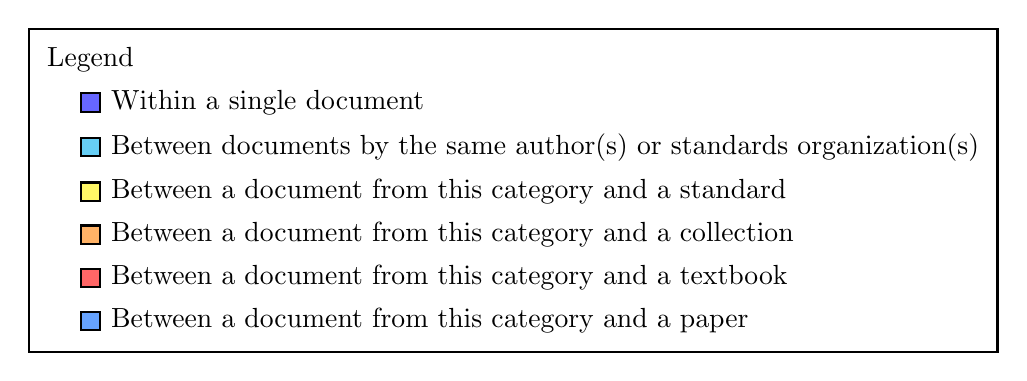
\begin{tikzpicture}
\matrix [thick, draw=black] {
\node[label=center:Legend] {{}}; \\
\node[thick, shape=rectangle, draw=black, fill=blue!60, label=right:{Within a single document}](0) {}; \\
\node[thick, shape=rectangle, draw=black, fill=cyan!60, label=right:{Between documents by the same author(s) or standards organization(s)}](1) {}; \\
\node[thick, shape=rectangle, draw=black, fill=yellow!60, label=right:{Between a document from this category and a standard}](2) {}; \\
\node[thick, shape=rectangle, draw=black, fill=orange!60, label=right:{Between a document from this category and a collection}](3) {}; \\
\node[thick, shape=rectangle, draw=black, fill=red!60, label=right:{Between a document from this category and a textbook}](4) {}; \\
\node[thick, shape=rectangle, draw=black, fill=blue!60!cyan!60, label=right:{Between a document from this category and a paper}](5) {}; \\
};
\end{tikzpicture}
\end{subfigure}
\end{center}
\hfill
\caption{Sources of discrepancies based on \hyperref[sources]{source tier}.}
\label{fig:discrepSources}
\end{figure*}
 \fi

\subsection{Discrepancy Classes}
\label{discrepClasses}

The following sections list observed discrepancies grouped by \emph{how} the
discrepancy manifests. These include \nameref{wrong}, \nameref{miss},
\nameref{contra}, \nameref{ambi}, \ifnotpaper \nameref{over}, and
    \nameref{redun}\else and \nameref{over}\fi.

\subsubsection{Mistakes}
\label{wrong}
\input{build/DiscrepClsWrong}

\subsubsection{Omissions}
\label{miss}
\input{build/DiscrepClsMiss}

\subsubsection{Contradictions}
\label{contra}
\input{build/DiscrepClsContra}

\subsubsection{Ambiguities}
\label{ambi}
\input{build/DiscrepClsAmbi}

\subsubsection{Overlaps}
\label{over}
\input{build/DiscrepClsOver}

\ifnotpaper
    \subsubsection{Redunancies}
    \label{redun}
    \input{build/DiscrepClsRedun}
\fi

\subsection{Discrepancy Categories}
\label{discrepCategories}

The following sections list observed discrepancies grouped by \emph{what area}
the discrepancy manifests in. These include \nameref{syns}, \nameref{pars},
\nameref{cats}, \nameref{defs}, \nameref{terms}, and \nameref{srcs}.

\subsubsection{Synonym Relation Discrepancies}
\label{syns}

The same approach often has many names. For example,
\emph{specification-based testing} is also called\todo{more in Umar2000}:
\begin{enumerate}
    \item Black-Box Testing
          \ifnotpaper
              (\citealp[p.~9]{IEEE2022}; \citeyear[p.~8]{IEEE2021};
              \citeyear[p.~431]{IEEE2017}; \citealp[p.~5-10]{SWEBOK2024};
              \citealpISTQB{}; \citealp[p.~46 (without hyphen)]{Firesmith2015};
              \citealp[p.~344]{SakamotoEtAl2013}; \citealp[p.~399]{vanVliet2000})
          \else
              \cite[p.~431]{IEEE2017}, \cite{ISTQB}, \cite[p.~5-10]{SWEBOK2024},
              \cite[p.~9]{IEEE2022}, \cite[p.~399]{vanVliet2000},
              \cite[p.~8]{IEEE2021}, % \cite[p.~46 (without hyphen)]{Firesmith2015},
              \cite[p.~344]{SakamotoEtAl2013}
          \fi
    \item Closed-Box Testing
          \ifnotpaper
              (\citealp[p.~9]{IEEE2022}; \citeyear[p.~431]{IEEE2017})
          \else
              \cite[p.~431]{IEEE2017}, \cite[p.~9]{IEEE2022}
          \fi
    \item Functional Testing\footnote{This may be an outlier; see
              \Cref{spec-func-test}.}
          \ifnotpaper
              (\citealp[p.~196]{IEEE2017}; \citealp[p.~44]{Kam2008};
              \citealp[p.~399]{vanVliet2000}; implied by \citealp[p.~129]{IEEE2021};
              \citeyear[p.~431]{IEEE2017})
          \else
              \cite[p.~196]{IEEE2017}, \cite[p.~399]{vanVliet2000},
              \cite[p.~44]{Kam2008}
          \fi
    \item Domain Testing \citep[p.~5-10]{SWEBOK2024}
          \ifnotpaper
    \item Input Domain-Based Testing \citetext{implied by
              \citealp[p.~4-8]{SWEBOK2014}}
          \fi
\end{enumerate}

While some of these synonyms may express mild variations, their core meaning
is nevertheless the same. Here we use the terms ``specification-based'' and
``structure-based testing'' as they articulate the source of the information
for designing test cases, but a team or project also using gray-box testing may
prefer the terms ``black-box'' and ``white-box testing'' for consistency.
Thus, synonyms do not inherently signify a discrepancy. Unfortunately, there
are many instances of incorrect or ambiguous synonyms, such as the following:

\input{build/DiscrepCatSyns}

\phantomsection{}
\label{multiSyns}
There are also cases in which a term is given a synonym to two (or more)
disjoint, unrelated terms, which would be a source of ambiguity to teams using
these terms. Ten of these cases were identified through automatic analysis of
the generated graphs\ifnotpaper, listed below\else. The following four are the
most prominent examples\fi:

% Moved here to display nicely in paper
\ifnotpaper\else\def\specfn{\seeFootAlways{spec-func-test}}

\begin{paperTable}
	\centering
	\caption{Pairs of test approaches with both child-parent and synonym relations.}
	\label{tab:parSyns}
	\begin{minipage}{\linewidth}
		\centering
		\begin{tabular}{|rcl|l|l|}
			\hline
			\ifnotpaper\rowcolor{McMasterMediumGrey}\fi
			\thead{``Child''}        & \thead{$\to$} & \thead{``Parent''}                       & \thead{Child-Parent Source(s)}                                        & \thead{Synonym Source(s)}                                                   \\
			\hline
			All Transitions Testing  & $\to$         & State Transition Testing                 & \citep[p.~19]{IEEE2021}                                               & \citep[p.~15]{Kam2008}                                                      \\
			Co-existence Testing     & $\to$         & Compatibility Testing                    & \cite[p.~3]{IEEE2022}, \cite{ISO_IEC2023a}, \cite[Tab.~A.1]{IEEE2021} & \citep[p.~37]{IEEE2021}                                                     \\
			Fault Tolerance Testing  & $\to$         & Robustness Testing\footnote{\ftrnote{F}} & \citep[p.~56]{Firesmith2015}                                          & \citepISTQB{}                                                               \\
			Functional Testing       & $\to$         & Specification-based Testing\specfn       & \citep[p.~38]{IEEE2021}                                               & \cite[p.~196]{IEEE2017}, \cite[p.~399]{vanVliet2000}, \cite[p.~44]{Kam2008} \\
			Orthogonal Array Testing & $\to$         & Pairwise Testing                         & \citep[p.~1055]{Mandl1985}                                            & \cite[p.~5-11]{SWEBOK2024}, \cite[p.~473]{Valcheva2013}                     \\
			Performance Testing      & $\to$         & Performance-related Testing              & \cite[p.~22]{IEEE2022}, \cite[p.~38]{IEEE2021}                        & \citep[p.~1187]{Moghadam2019}                                               \\
			Use Case Testing         & $\to$         & Scenario Testing                         & \cite[p.~20]{IEEE2021}\todo{OG Hass, 2008}                            & \cite{ISTQB}, \cite[pp.~47-49]{Kam2008}                                     \\
			\hline
		\end{tabular}
	\end{minipage}
\end{paperTable}
\fi

\begin{enumerate}
    \item \textbf{Invalid Testing:}
\begin{itemize}
    \item Error Tolerance Testing \citep[p.~45]{Kam2008}
    \item Negative Testing \ifnotpaper
              (\citealpISTQB{}; implied by \citealp[p.~10]{IEEE2021}) \else
              \citep{ISTQB} (implied by \citep[p.~10]{IEEE2021}) \fi
\end{itemize}
\item \textbf{Soak Testing:}
\begin{itemize}
    \item Endurance Testing \citep[p.~39]{IEEE2021}
    \item Reliability Testing\ifnotpaper\
              (\citealp[Tab.~2]{Gerrard2000a}; \citeyear[Tab.~1,~p.~26]{Gerrard2000b})
          \else\footnote{Endurance testing is given as a kind of reliability
                  testing by \citet[p.~55]{Firesmith2015}, although the terms
                  are not synonyms.} \citep[Tab.~1,~p.~26]{Gerrard2000b},
              \citep[Tab.~2]{Gerrard2000a}\fi
\end{itemize}
\item \textbf{User Scenario Testing:}
\begin{itemize}
    \item Scenario Testing \citepISTQB{}
    \item Use Case Testing\ifnotpaper\ \else\footnote{``Scenario testing'' and
                  ``use case testing'' are given as synonyms by \citepISTQB{}
                  and \citep[pp.~47-49]{Kam2008}
                  but listed separately by \citep[p.~22]{IEEE2022}, \ifnotpaper who
                      also give \else which also gives \fi ``use case testing'' as a
                  ``common form of scenario testing'' \citep[p.~20]{IEEE2021}.
                  This implies that ``use case testing'' may instead be a child of
                  ``user scenario testing'' (see \Cref{tab:parSyns}).}\fi
          \citep[p.~48]{Kam2008} (although ``an actor can be a user or another
          system'' \citep[p.~20]{IEEE2021})
\end{itemize}
\item \textbf{Link Testing:}
\begin{itemize}
    \item Branch Testing (implied by \citealp[p.~24]{IEEE2021})
    \item Component Integration Testing \citep[p.~45]{Kam2008}
    \item Integration Testing (implied by \citealp[p.~13]{Gerrard2000a})
\end{itemize}
\end{enumerate}

\subsubsection{Parent-Child Relation Discrepancies}
\label{pars}

\nameref{par-chd-rels} are also not immune to difficulties\ifnotpaper, as shown
by the following discrepancies:
\input{build/DiscrepCatPars} \else; for example, performance \fi testing and
security testing are given as subtypes of reliability testing by
\citep{ISO_IEC2023a}, but these are all listed separately by
\citep[p.~53]{Firesmith2015}.

\phantomsection{}\label{selfPars}
Additionally, some self-referential definitions imply that a test
approach is a parent of itself. Since these are by nature self-contained within
a given source, these are counted \emph{once} as explicit discrepancies within
their sources in \Cref{tab:discreps}. \ifnotpaper The following examples were
    identified through automatic analysis of the generated graphs:
    \input{build/selfCycles} Interestingly, performance testing is \emph{not}
    described as a sub-approach of usability testing by \citep{Gerrard2000a,
        Gerrard2000b}, which would have been more meaningful information to
    capture. \else For example, performance and usability testing are both
    given as sub-approaches of themselves \cite[Tab.~2]{Gerrard2000a},
    \cite[Tab.~1]{Gerrard2000b}.\fi

There are also pairs of synonyms where one is described as a
sub-approach of the other, abusing the meaning of ``synonym'' and
causing confusion. We identified \parSynCount{} of these pairs through automatic
analysis of the generated graphs, \ifnotpaper which are \else with the most
    prominent \fi given in \Cref{tab:parSyns}.
\ifnotpaper Finally, it is worth pointing out that \ftrnote{f}

    \begin{landscape}
        \discrepsTable{}
        \def\specfn{\seeFootAlways{spec-func-test}}

\begin{paperTable}
	\centering
	\caption{Pairs of test approaches with both child-parent and synonym relations.}
	\label{tab:parSyns}
	\begin{minipage}{\linewidth}
		\centering
		\begin{tabular}{|rcl|l|l|}
			\hline
			\ifnotpaper\rowcolor{McMasterMediumGrey}\fi
			\thead{``Child''}        & \thead{$\to$} & \thead{``Parent''}                       & \thead{Child-Parent Source(s)}                                        & \thead{Synonym Source(s)}                                                   \\
			\hline
			All Transitions Testing  & $\to$         & State Transition Testing                 & \citep[p.~19]{IEEE2021}                                               & \citep[p.~15]{Kam2008}                                                      \\
			Co-existence Testing     & $\to$         & Compatibility Testing                    & \cite[p.~3]{IEEE2022}, \cite{ISO_IEC2023a}, \cite[Tab.~A.1]{IEEE2021} & \citep[p.~37]{IEEE2021}                                                     \\
			Fault Tolerance Testing  & $\to$         & Robustness Testing\footnote{\ftrnote{F}} & \citep[p.~56]{Firesmith2015}                                          & \citepISTQB{}                                                               \\
			Functional Testing       & $\to$         & Specification-based Testing\specfn       & \citep[p.~38]{IEEE2021}                                               & \cite[p.~196]{IEEE2017}, \cite[p.~399]{vanVliet2000}, \cite[p.~44]{Kam2008} \\
			Orthogonal Array Testing & $\to$         & Pairwise Testing                         & \citep[p.~1055]{Mandl1985}                                            & \cite[p.~5-11]{SWEBOK2024}, \cite[p.~473]{Valcheva2013}                     \\
			Performance Testing      & $\to$         & Performance-related Testing              & \cite[p.~22]{IEEE2022}, \cite[p.~38]{IEEE2021}                        & \citep[p.~1187]{Moghadam2019}                                               \\
			Use Case Testing         & $\to$         & Scenario Testing                         & \cite[p.~20]{IEEE2021}\todo{OG Hass, 2008}                            & \cite{ISTQB}, \cite[pp.~47-49]{Kam2008}                                     \\
			\hline
		\end{tabular}
	\end{minipage}
\end{paperTable}

    \end{landscape}
\else % Moved earlier to display nicely in paper
\fi

\subsubsection{Test Approach Category Discrepancies}
\label{cats}

While the IEEE categorization of testing approaches described in
\refIEEETestTerms{} is useful, it
is not without its faults. The boundaries between items within a category may
be unclear: ``although each technique is defined independently of all others,
in practice [sic] some can be used in combination with other techniques''
\citep[p.~8]{IEEE2021}. For example, ``the test coverage items derived by
applying equivalence partitioning can be used to identify the input parameters
of test cases derived for scenario testing'' \citetext{p.~8}. Even the categories
themselves are not consistently defined, and some approaches are categorized
differently by different sources:

% ; these differences are tracked so
% they can be analyzed more systematically\seeThesisIssuePar{21}.

\input{build/DiscrepCatCats}

There are also instances of inconsistencies between parent and child
test approach categorizations. This may indicate they aren't necessarily the
same, or that more thought must be given to this method of classification.

\subsubsection{Definition Discrepancies}
\label{defs}

Perhaps the most interesting category for those seeking to understand how to
apply a given test approach, there are many discrepancies between how test
approaches, as well as supporting terms, are defined:

\input{build/DiscrepCatDefs}

% TODO: re-investigate this after going through the rest of ISO/IEC/IEEE 29119
\ifnotpaper
    Also of note: \citep{IEEE2022, IEEE2021}, from the
    ISO/IEC/IEEE 29119 family of standards, mention the following 23 test
    approaches without defining them. This means that out of the 114 test
    approaches they mention, about 20\% have no associated definition!

    However, the previous version of this standard, \citeyearpar{IEEE2013},
    generally explained two, provided references for two, and explicitly defined
    one of these terms, for a total of five definitions that could (should) have
    been included in \citeyearpar{IEEE2022}! These terms have been
    \underline{underlined}\ifnotpaper%
        , \emph{italicized}, and \textbf{bolded}, respectively%
    \fi. Additionally, entries marked with an asterisk* were defined (at least
    partially) in \citeyearpar{IEEE2017}, which would have been available when
    creating this family of standards. These terms bring the total count of terms
    that could (should) have been defined to nine; almost 40\% of undefined test
    approaches could have been defined!

    \begin{itemize}
        \item \underline{Acceptance Testing*}
        \item Alpha Testing*
        \item Beta Testing*
        \item Capture-Replay Driven Testing
        \item Data-driven Testing
        \item Error-based Testing
        \item Factory Acceptance Testing
        \item Fault Injection Testing
        \item Functional Suitability Testing (also mentioned but not defined in
              \citep{IEEE2017})
        \item \underline{Integration Testing}*
        \item Model Verification
        \item Operational Acceptance Testing
        \item Orthogonal Array Testing
        \item Production Verification Testing
        \item Recovery Testing* (Failover/Recovery Testing, Back-up/Recovery
              Testing, \formatPaper{\textbf}{Backup and Recovery Testing*},
              Recovery*;\seeAlways{recov-discrep})
        \item Response-Time Testing
        \item \formatPaper{\emph}{Reviews} (ISO/IEC 20246) (Code Reviews*)
        \item Scalability Testing (defined as a synonym of ``capacity
              testing'';\seeAlways{scal-discrep})
        \item Statistical Testing
        \item System Integration Testing (System Integration*)
        \item System Testing* (also mentioned but not defined in \citep{IEEE2013})
        \item \formatPaper{\emph}{Unit Testing*}
              (IEEE Std 1008-1987, IEEE Standard for
              Software Unit Testing implicitly listed in the bibliography!)
        \item User Acceptance Testing
    \end{itemize}
\fi

\subsubsection{Terminology Discrepancies}
\label{terms}

While some discrepancies exist because the definition of a term is wrong,
others exist because term's \emph{name} or \emph{label} is wrong! This could be
considered a ``sister'' category of \nameref{defs}, but these
discrepancies seemed different enough to merit their own category. \ifnotpaper
    This most often manifests as terms that are included in reference material
    that should not have been, terms that share the same acronym, and terms
    that have typos or are redundant. \fi The following \ifnotpaper
    discrepancies are presented in that order\else are examples of these
    discrepancies\fi:

\input{build/DiscrepCatTerms}

\subsubsection{Source Discrepancies}
\label{srcs}

Sometimes a source cites another for a piece of information that does not
appear! \ifnotpaper
    The following discrepancies are examples of this:
    \input{build/DiscrepCatSrcs}
\else
    For example, \citet[p.~184]{DoğanEtAl2014} \multAuthHelper{claim} that
    \citet{SakamotoEtAl2013} \multAuthHelper{define} ``prime path coverage'',
    but it does not.
\fi


\subsection{Functional Testing}
\label{func-test-discrep}

``Functional testing'' is described alongside many other, likely related,
terms. This leads to confusion about what distinguishes these terms, as shown
by the following five:

\subsubsection{Specification-based Testing}
\label{spec-func-test}
This is defined as ``testing in which the principal test basis is the external
inputs and outputs of the test item'' \citep[p.~9]{IEEE2022}. This agrees
with a definition of ``functional testing'': ``testing that
\dots\ focuses solely on the outputs generated in response to
selected inputs and execution conditions'' \citep[p.~196]{IEEE2017}.
\todo{\citet[p.~399]{vanVliet2000} may list these as synonyms; investigate}
Notably, \citet{IEEE2017} lists both as synonyms of
``black-box testing'' \citetext{pp. 431, 196, respectively}, despite them
sometimes being defined separately. For example, the \acf{istqb} defines
``specification-based testing'' as ``testing based on an analysis of the
specification of the component or system'' \ifnotpaper (and gives ``black-box
    testing'' as a synonym) \fi and ``functional testing'' as ``testing
performed to evaluate if a component or system satisfies functional
requirements'' \ifnotpaper (specifying no synonyms) \citepISTQB{};
    % Discrep count (SYNS, CONTRA): {IEEE2022} {IEEE2017} | ISTQB
    the latter references \citet[p.~196]{IEEE2017}
    (``testing conducted to evaluate the compliance of a system or
    component with specified functional requirements'') which
    \emph{has} ``black-box testing'' as a synonym, and mirrors
    \citet[p.~21]{IEEE2022} (testing ``used to check the implementation
    of functional requirements'')\else \cite{ISTQB}\fi. Overall,
specification-based testing \citep[pp.~2-4,~6-9,~22]{IEEE2022} \ifnotpaper and
    black-box testing (\citealp[p.~5-10]{SWEBOK2024};
    \citealp[p.~3]{SouzaEtAl2017})
    % \else \cite[p.~3]{SouzaEtAl2017}, \cite[p.~5-10]{SWEBOK2024}
    are test design techniques \else is a test design technique \fi used to
``derive corresponding test cases'' \citep[p.~11]{IEEE2022} from
``selected inputs and execution conditions'' \citep[p.~196]{IEEE2017}.

\subsubsection{Correctness Testing}
\ifnotpaper \citeauthor{SWEBOK2024} \else The \acs{swebok} V4 \fi says
``test cases can be designed to check that the functional
specifications are correctly implemented, which is variously
referred to in the literature as conformance testing, correctness
testing or functional testing'' \ifnotpaper \citeyearpar[p.~5-7]{SWEBOK2024}%
\else \cite[p.~5-7]{SWEBOK2024}\fi; this mirrors previous definitions
of ``functional testing'' \ifnotpaper (\citealp[p.~21]{IEEE2022};
    \citeyear[p.~196]{IEEE2017}) \else \cite[p.~196]{IEEE2017},
    \cite[p.~21]{IEEE2022} \fi but groups it with ``correctness
testing''. Since ``correctness'' is a software quality \ifnotpaper
    (\citealp[p.~104]{IEEE2017}; \citealp[p.~3-13]{SWEBOK2024}) \else
    \cite[p.~104]{IEEE2017}, \cite[p.~3-13]{SWEBOK2024} \fi which is
what defines a ``test type'' \citep[p.~15]{IEEE2022}\ifnotpaper\
    (see \Cref{qual-test})\fi,
it seems consistent to label ``functional testing'' as a ``test type''
\citep[pp.~15,~20,~22]{IEEE2022}; this conflicts with its categorization
as a ``technique'' if considered a synonym of \nameref{spec-func-test}.
% Discrep count (CATS, CONTRA): implied by {IEEE2017} {SWEBOK2024} {IEEE2022} | {IEEE2022} {SWEBOK2024} {SouzaEtAl2017} {IEEE2017}
``Correctness testing'' is listed separately from ``functionality testing'' by
\citet[p.~53]{Firesmith2015}.
% Discrep count (SYNS, CONTRA): {SWEBOK2024} | {Firesmith2015}

\subsubsection{Conformance Testing}
Testing that ensures ``that the functional specifications are correctly
implemented'', and can be called ``conformance testing'' or ``functional
testing'' \citep[p.~5-7]{SWEBOK2024}.
``Conformance testing'' is later defined as testing used ``to
verify that the \acs{sut} conforms to standards, rules,
specifications, requirements, design, processes, or practices''
\citep[p.~5-7]{SWEBOK2024}. This definition seems to be a superset
of testing methods mentioned earlier as the latter includes ``standards,
rules, requirements, design, processes, \dots\ [and]'' practices in
\emph{addition} to specifications!
% Discrep count (SYNS, OVER): {SWEBOK2024} | implied by {SWEBOK2024}

A complicating factor is that ``compliance testing'' is also
(plausibly) given as a synonym of ``conformance testing''
\citep[p.~43]{Kam2008}. However, ``conformance
testing'' can also be defined as testing that evaluates the degree
to which ``results \dots\ fall within the limits that define
acceptable variation for a quality requirement''
\citep[p.~93]{IEEE2017}\todo{OG PMBOK 5th ed.}, which seems to
describe something different.
% Discrep count (SYNS, AMBI): {Kam2008} | implied by {IEEE2017}

% TODO: pull out into Recommendations
% Perhaps this second definition of
% ``conformance testing'' should be used, and the previous definition
% of ``compliance testing'' should be used for describing compliance with
% external standards, rules, etc.~to keep them distinct.

\subsubsection{Functional Suitability Testing}
Procedure testing is
called a ``type of functional suitability testing''
\citep[p.~7]{IEEE2022} but no definition of that term is given.
``Functional suitability'' is the
``capability of a product to provide functions that meet stated and
implied needs of intended users when it is used under specified
conditions'', including meeting ``the functional specification''
\citep{ISO_IEC2023a}. This seems to align with the definition of
``functional testing'' as related to ``black-box/%
specification-based testing''.
\ifnotpaper
    ``Functional suitability'' has
    three child terms: ``functional completeness'' (the ``capability of
    a product to provide a set of functions that covers all the
    specified tasks and intended users' objectives''), ``functional
    correctness'' (the ``capability of a product to provide accurate
    results when used by intended users''), and ``functional
    appropriateness'' (the ``capability of a product to provide
    functions that facilitate the accomplishment of specified tasks and
    objectives'') \citep{ISO_IEC2023a}. Notably, ``functional
    correctness'', which includes precision and accuracy
    (\citealp{ISO_IEC2023a}; \citealpISTQB{}), \else ``Functional
    correctness'', a child of ``functional suitability'', is the ``capability
    of a product to provide accurate results when used by intended users''
    \cite{ISO_IEC2023a} and \fi seems to align with
the quality/ies that would be tested by ``correctness'' testing.

\subsubsection{Functionality Testing}
``Functionality'' is defined as the
``capabilities of the various \dots\ features provided by a product''
\citep[p.~196]{IEEE2017} and is said to be a synonym of
``functional suitability'' \citepISTQB{}, although it seems
like it should really be a synonym of ``functional completeness'' based on
\citep{ISO_IEC2023a}, which would make ``functional suitability'' a
% Discrep count (SYNS, CONTRA): ISTQB | implied by {ISO_IEC2023a}
sub-approach. Its associated test type
is implied to be a sub-approach of build verification testing
\citepISTQB{} and made distinct from ``functional testing''%
\ifnotpaper; interestingly, security is described as a sub-approach of both
non-functional and functionality testing\fi\ \citep[Tab.~2]{Gerrard2000a}.
``Functionality testing'' is listed separately from ``correctness testing'' by
\citet[p.~53]{Firesmith2015}.

\ifnotpaper
    \subsection[Operational (Acceptance) Testing (OAT)]{\acf{operat}}
    \label{oat-discrep}
    % Discrep count (TERMS, CONTRA): {IEEE2022} ISTQB | {SWEBOK2024} {ISO_IEC2018} {IEEE2017} {SWEBOK2014}
    % Discrep count (SYNS, CONTRA): {LambdaTest2024} {BocchinoAndHamilton1996} | {Firesmith2015}
    Some sources refer to ``operational acceptance testing'' (\citealp[p.~22]{IEEE2022};
    \citealpISTQB{}) while some refer to ``operational testing''
    (\citealp[p.~6-9,~in the context of software engineering operations]{SWEBOK2024};
    \citealp{ISO_IEC2018}; \citealp[p.~303]{IEEE2017};
    \citealp[pp.~4-6,~4-9]{SWEBOK2014}). A distinction is sometimes made
    \citep[p.~30]{Firesmith2015} but without accompanying definitions, it is hard
    to evaluate its merit. Since this terminology is not standardized, I
    propose that the two terms are treated as synonyms (as done by other sources
    \citep{LambdaTest2024, BocchinoAndHamilton1996}) as a type of
    acceptance testing (\citealp[p.~22]{IEEE2022}; \citealpISTQB{}) that focuses on
    ``non-functional'' attributes of the system \citep{LambdaTest2024}%
    \todo{find more academic sources}.
    %% Recommendations in the above: should be split out

    %% The following 'summary' appears out of place? I'm not quite understanding
    % the point this is trying to make.
    A summary of definitions of ``operational (acceptance) testing'' is that
    it is ``test[ing] to determine the correct
    installation, configuration and operation of a module and that it operates
    securely in the operational environment'' \citep{ISO_IEC2018} or ``evaluate a
    system or component in its operational environment'' \citep[p.~303]{IEEE2017},
    particularly ``to determine if operations and/or systems administration staff
    can accept [it]'' \citepISTQB{}.
\fi

\subsection{Recovery Testing}
\label{recov-discrep}

``Recovery testing'' is ``testing \dots\ aimed at verifying
software restart capabilities after a system crash or other disaster''
\citep[p.~5-9]{SWEBOK2024} including ``recover[ing] the data directly affected
and re-establish[ing] the desired state of the system''
\ifnotpaper
    (\citealp{ISO_IEC2023a}; similar in \citealp[p.~7-10]{SWEBOK2024})
\else
    \cite{ISO_IEC2023a} (similar in \cite[p.~7-10]{SWEBOK2024})
\fi
so that the system ``can perform required functions'' \citep[p.~370]{IEEE2017}.
It is also called ``recoverability testing'' \cite[p.~47]{Kam2008} and
potentially ``restart \& recovery (testing)'' \cite[Fig.~5]{Gerrard2000a}.
% Discrep count (SYNS, AMBI): {Gerrard2000a}
The following terms, along with ``recovery testing'' itself
\citep[p.~22]{IEEE2022} are all classified as test types, and the relations
between them can be found in \Cref{fig:recovery-graph-current}.

%% again, maybe convert to \paragraph ?
\begin{itemize}
    \item \textbf{Recoverability Testing:} Testing ``how well a system or
          software can recover data during an interruption or failure''
          \ifnotpaper
              (\citealp[p.~7-10]{SWEBOK2024}; similar in \citealp{ISO_IEC2023a})
          \else
              \cite[p.~7-10]{SWEBOK2024} (similar in \cite{ISO_IEC2023a})
          \fi
          and ``re-establish the desired state of the system'' \citep{ISO_IEC2023a}.
          Synonym for ``recovery testing'' in \citet[p.~47]{Kam2008}.
    \item \textbf{Disaster/Recovery Testing} serves to evaluate if a system
          can ``return to normal operation after a hardware
          or software failure'' \citep[p.~140]{IEEE2017} or if ``operation of
          the test item can be transferred to a different operating site and
          \dots\ be transferred back again once the failure has been
          resolved'' \citeyearpar[p.~37]{IEEE2021}. These two definitions seem to
          describe different aspects of the system, where the first is
          intrinsic to the hardware/software and the second might not be.
          % Discrep count (DEFS, OVER): {IEEE2017} | {IEEE2021}
    \item \textbf{Backup and Recovery Testing} ``measures the
          degree to which system state can be restored from backup within
          specified parameters of time, cost, completeness, and accuracy in
          the event of failure'' \citep[p.~2]{IEEE2013}. This may be what is
          meant by ``recovery testing'' in the context of performance-related
          testing and seems to correspond to the definition of
          ``disaster/recovery testing'' in \citeyearpar[p.~140]{IEEE2017}.
    \item \textbf{Backup/Recovery Testing:} Testing that determines the
          ability ``to restor[e] from back-up memory in the event of failure,
          without transfer[ing] to a different operating site or back-up
          system'' \citep[p.~37]{IEEE2021}. This seems to correspond to the
          definition of ``disaster/recovery testing'' in
          \citeyearpar[p.~37]{IEEE2021}. It is also given as a sub-type of
          ``disaster/recovery testing'', even though that tests if ``operation
          of the test item can be transferred to a different operating site''
          \citetext{p.~37}. % Discrep count (PARS, CONTRA): {IEEE2021} | {IEEE2021}
          It also seems to overlap with ``backup and
          recovery testing'', which adds confusion.
          % Discrep count (DEFS, OVER): {IEEE2021} | {IEEE2013}
    \item \textbf{Failover/Recovery Testing:} Testing that determines the
          ability ``to mov[e] to a back-up system in the event of failure,
          without transfer[ing] to a different operating site''
          \citep[p.~37]{IEEE2021}. This is given as a sub-type of
          ``disaster/recovery testing'', even though that tests if ``operation
          of the test item can be transferred to a different operating site''
          \citetext{p.~37}. % Discrep count (PARS, CONTRA): {IEEE2021} | {IEEE2021}
    \item \textbf{Failover Testing:} Testing that ``validates the SUT's
          ability to manage heavy loads or unexpected failure to continue
          typical operations'' \citep[p.~5-9]{SWEBOK2024} by entering a
          ``backup operational mode in which [these responsibilities] \dots\
          are assumed by a secondary system'' \citepISTQB{}. While not
          \emph{explicitly} related to recovery, ``failover/recovery testing''
          also describes the idea of ``failover'', and \citet[p.~56]{Firesmith2015}
          uses the term ``failover and recovery testing'', which could be a
          synonym of both of these terms.
          % Discrep count (SYNS, AMBI): {SWEBOK2024} ISTQB | implied by {Firesmith2015}
\end{itemize}

\subsection{Scalability Testing}
\label{scal-discrep}

There were three ambiguities around the term ``scalability testing'', listed
below. The relations between these test approaches (and other relevant ones)
are shown in \Cref{fig:scal-graph-current}.

\begin{enumerate}
    \item % Discrep count (SYNS, CONTRA): {IEEE2021} | {Firesmith2015} {Bas2024}
          \ifnotpaper \citeauthor{IEEE2021} \else ISO/IEC and IEEE \fi give
          ``scalability testing'' as a synonym of ``capacity testing''
          \ifnotpaper \citeyearpar[p.~39]{IEEE2021} \else \cite[p.~39]{IEEE2021}
          \fi while other sources differentiate between the two
          \ifnotpaper \citetext{\citealp[p.~53]{Firesmith2015};
                  \citealp[pp.~22-23]{Bas2024}}
          \else \citep[p.~53]{Firesmith2015}, \citep[pp.~22-23]{Bas2024}
          \fi
    \item % Discrep count (DEFS, CONTRA): {IEEE2021} | implied by {ISO_IEC2023a}
          \ifnotpaper \citeauthor{IEEE2021} \else ISO/IEC and IEEE \fi give
          the external modification of the system as part of ``scalability''
          \ifnotpaper \citeyearpar[p.~39]{IEEE2021}\else
              \cite[p.~39]{IEEE2021}\fi, while \citet{ISO_IEC2023a} \ifnotpaper
              imply \else implies \fi that it is limited to the system itself
    \item % Discrep count (TERMS, WRONG): {SWEBOK2024}
          The \acs{swebok} V4's definition of ``scalability testing''
          \citep[p.~5-9]{SWEBOK2024} is really a definition of usability
          testing!
\end{enumerate}

% \subsection{Performance Testing}
% \label{perf-test-ambiguity}

% Similarly, ``performance'' and ``performance efficiency'' are both given as
% software qualities by \ifnotpaper\citeauthor{IEEE2017}\else
%       \cite[p.~319]{IEEE2017}\fi, with the latter defined as the ``performance
% relative to the amount of resources used under stated conditions''
% \ifnotpaper\citeyearpar[p.~319]{IEEE2017} \fi or the ``capability of a product
% to perform its functions within specified time and throughput parameters and be
% efficient in the use of resources under specified conditions'' \citep{ISO_IEC2023a}.
% Initially, there didn't seem to be any meaningful distinction between the two,
% although the term ``performance testing'' is defined
% \ifnotpaper\citeyearpar[p.~320]{IEEE2017}\else\citetext{p.~320}\fi\
% and used by \ifnotpaper\citeauthor{IEEE2017}\else\cite{IEEE2017}\fi\ and the term
% ``performance efficiency testing'' is \emph{also} used by
% \ifnotpaper\citeauthor{IEEE2017}\else\cite{IEEE2017}\fi\ (but not defined
% explicitly). \ifnotpaper Further discussion\seeThesisIssuePar{43} brought us to
%       the conclusion \else It can then be concluded \fi that ``performance
% efficiency testing'' is a subset of ``performance testing'', and the
% difference of ``relative to the amount of resources used'' or ``be efficient in
% the use of resources'' between the two is meaningful.

\subsection{Compatibility Testing}
\label{compat-discrep}

% Discrep count (DEFS, OVER): {IEEE2022} | {IEEE2017} ISTQB {ISO_IEC2023a}
``Compatibility testing'' is defined as ``testing that measures the
degree to which a test item can function satisfactorily alongside
other independent products in a shared environment (co-existence),
and where necessary, exchanges information with other systems or
components (interoperability)'' \citep[p.~3]{IEEE2022}. This
definition is nonatomic as it combines the ideas of ``co-existence''
and ``interoperability''. The term ``interoperability testing'' is
not defined, but is used three times \citep[pp.~22,~43]{IEEE2022}
% Discrep count (TERMS, WRONG): {IEEE2022}
(although the third usage seems like it should be ``portability
testing''). This implies that ``co-existence testing'' and
``interoperability testing'' should be defined as their own terms,
which is supported by definitions of ``co-existence'' and
``interoperability'' often being separate \ifnotpaper
    \citetext{\citealpISTQB{}; \citealp[pp.~73,~237]{IEEE2017}}%
\else
    \cite[pp.~73,~237]{IEEE2017}, \cite{ISTQB}%
\fi, the definition of
``interoperability testing'' from \citet[p.~238]{IEEE2017},
and the decomposition of ``compatibility'' into ``co-existence''
and ``interoperability'' by \citet{ISO_IEC2023a}!
% Discrep count (SYNS, WRONG): implied by {IEEE2021} | {IEEE2022}
The ``interoperability'' element of ``compatibility testing'' is explicitly
excluded by \citet[p.~37]{IEEE2021}, (incorrectly) implying that ``compatibility
testing'' and ``co-existence testing'' are synonyms.
% Discrep count (SYNS, AMBI): {Kam2008} | {IEEE2022}
Furthermore, the definition of ``compatibility testing'' in
\citep[p.~43]{Kam2008} unhelpfully says ``See \emph{interoperability testing}'',
adding another layer of confusion to the direction of their relationship.

\ifnotpaper
    \subsection{Inferred Discrepancies}
    \label{infer-discreps}
    Along the course of this analysis, we inferred many potential discrepancies.
    Some of these have a conflicting source while others do not. These are
    excluded from any counts of the numbers of discrepancies, since they are
    more subjective, but are given below for completeness.

    \subsubsection{Inferred Synonym Discrepancies}
    See \Cref{multiSyns}.

    \begin{enumerate}
        \input{build/infMultiSyns}
    \end{enumerate}

    Additionally, \citet[p.~46]{Kam2008} gives ``program testing'' as a synonym
    of ``component testing'' but it probably should be a synonym of ``system
    testing'' instead.
    % \item \refHelper \citet[p.~46]{Kam2008} gives ``program testing'' as a
    % synonym of ``component testing'' but it probably should be a synonym of
    % ``system testing'' instead.

    \subsubsection{Inferred Parent Discrepancies}
    As in \Cref{tab:parSyns}, some discrepancies occur when test approaches
    are classified as both children/parents \emph{and} synonyms. The first two
    lists below give approaches that are given one of these relations by at
    least one source when it may make more sense for them to have the other
    relation. The third list gives approaches that could be inferred to have
    either relation, so more thought would have to be given before a
    recommendation can be made.

    \input{build/infParSyns}

    Additionally, \citep[Tab.~2]{Gerrard2000a} does \emph{not} give
    ``functionality testing'' as a parent of ``end-to-end functionality testing''.
    % \item \refHelper \citep[Tab.~2]{Gerrard2000a} does \emph{not} give
    % ``functionality testing'' as a parent of ``end-to-end functionality testing''.

    \subsubsection{Other Inferred Discrepancies}
    The following are discrepancies that, if were more concrete, would also be
    included alongside the other discrepancies:
    \begin{itemize}
        \item ``Fuzz testing'' is ``tagged'' (?) as ``artificial
              intelligence'' \citep[p.~5]{IEEE2022}.
        \item \citeauthor{Gerrard2000b}'s definition for ``security
              audits'' seems too specific, only applying to ``the products
              installed on a site'' and ``the known vulnerabilities for
              those products'' \citeyearpar[p.~28]{Gerrard2000b}.
    \end{itemize}
\fi
\section{Recommendations}\label{recs}

As we have shown in \Cref{flaws}, ``testing is a mess'' \citetext{Mosser,
    2023, priv.\ comm.}! It will take a lot of time, effort, expertise, and
training to organize these terms (and their relations) logically. However, the
hardest step is often the first one, so we attempt to give some examples of how
this ``rationalization'' can occur. These changes often arise when we notice an
issue with the current state of the terminology and think about what \emph{we}
would do to make it better. We do not claim that these are correct, unbiased,
or exclusive, just that they can be used as an inspiration for those wanting to
pick up where we leave off.

When redefining terms, we seek to make them:
\begin{enumerate}
    \item Atomic (e.g., disaster/recovery testing seems to have two
          disjoint definitions)
    \item Straightforward (e.g., backup and recovery testing's definition
          implies the idea of performance, but its name does not
          \ifnotpaper; failover/recovery testing, failover and recovery
          testing, and failover testing are all given separately\fi)
    \item Consistent (e.g., backup/recovery testing and failover/recovery
          testing explicitly exclude an aspect included in its parent
          disaster/recovery testing)
\end{enumerate}
Likewise, we seek to eliminate classes of flaws that can be detected
automatically, such as test approaches that are given as synonyms to multiple
distinct approaches (\Cref{multiSyns}) or as parents of themselves
(\Cref{selfPars}), or pairs of approaches with both a parent-child \emph{and}
synonym relation (\Cref{parSyns}).\todo{Same label to different phantomsections;
    is that OK?}

We give recommendations for the areas of \ifnotpaper operational (acceptance)
    testing (\Cref{oat-test-rec}), \fi recovery testing (\Cref{rec-test-rec}),
scalability testing (\Cref{scal-test-rec}), and performance-related testing
(\Cref{perf-test-rec}). Graphical representations (described in
\Cref{\ifnotpaper graph-gen\else tools\fi}) of these subsets are given in
\recFigs{}, in which arrows representing relations between approaches are
coloured based on the source tier (see \Cref{sources}) that defines them.
Any added approaches or relations are colored \textcolor{orange}{orange}.
\ifnotpaper Note that
    inferred relations (colored \textcolor{gray}{grey}) are included for
    completeness\todo{Should this be the case?}, despite not coming from the
    literature (see \Cref{infers}).

    \subsection{Operational (Acceptance) Testing}\label{oat-test-rec}
    Since this terminology is not standardized (see \Cref{oat-flaw}), we
    propose that ``\acf{operat}'' and ``\acf{ot}'' are treated as
    synonyms for a type of acceptance testing (\citealp[p.~22]{IEEE2022};
    \citealpISTQB{}) that focuses on ``non-functional'' attributes of the system
    \citep{LambdaTest2024}\todo{find more academic sources}. Indeed, this is how we
    track this approach in \ourApproachGlossary{}! We define it as ``test[ing] to
    determine the correct installation, configuration and operation of a module and
    that it operates securely in the operational environment'' \citep{ISO_IEC2018}
    or to ``evaluate a system or component in its operational environment''
    \citep[p.~303]{IEEE2017}, particularly ``to determine if operations and/or
    systems administration staff can accept [it]'' \citepISTQB{}.
\fi

\subsection{Recovery Testing}\label{rec-test-rec}
The following terms should be used in place of the current terminology to
more clearly distinguish between different recovery-related test approaches.
The result of the proposed terminology, along with their relations, is
demonstrated in \Cref{fig:recovery-graph-proposed}.

\recoveryGraphs{}

\begin{itemize}
    \item \textbf{Recoverability Testing:} ``Testing \dots\ aimed at
          verifying software restart capabilities after a system crash or
          other disaster'' \citep[p.~5-9]{SWEBOK2024} including ``recover[ing]
          the data directly affected and re-establish[ing] the desired state
          of the system''
          \ifnotpaper
              (\citealp{ISO_IEC2023a}; similar in \citealp[p.~7-10]{SWEBOK2024})
          \else
              \cite{ISO_IEC2023a} (similar in \cite[p.~7-10]{SWEBOK2024})
          \fi so that the system ``can perform
          required functions'' \citep[p.~370]{IEEE2017}. ``Recovery testing''
          will be a synonym, as in \citep[p.~47]{Kam2008}, since it is the
          more prevalent term throughout various sources, although
          ``recoverability testing'' is preferred to indicate that this
          explicitly focuses on the \emph{ability} to
          recover, not the \emph{performance} of recovering.
    \item \textbf{Failover Testing:} Testing that ``validates the SUT's
          ability to manage heavy loads or unexpected failure to continue
          typical operations'' \cite[p.~5-9]{SWEBOK2024} by entering a
          ``backup operational mode in which [these responsibilities] \dots\
          are assumed by a secondary system'' \citepISTQB{}. This will
          replace ``failover/recovery testing'', since it is more clear, and
          since this is one way that a system can recover from failure, it
          will be a subset of ``recovery testing''.
    \item \textbf{Transfer Recovery Testing:} Testing to evaluate if,
          in the case of a failure, ``operation of the test item can be
          transferred to a different operating site and \dots\ be transferred
          back again once the failure has been resolved''
          \citeyearpar[p.~37]{IEEE2021}. This replaces the second definition
          of ``disaster/recovery testing'', since the first is just a
          description of ``recovery testing'', and could potentially be
          considered as a kind of failover testing. This may not be
          intrinsic to the hardware/software (e.g., may be the responsibility
          of humans/processes).
    \item \textbf{Backup Recovery Testing:} Testing that determines the
          ability ``to restor[e] from back-up memory in the event of failure''
          \citep[p.~37]{IEEE2021}. The qualification that this occurs
          ``without transfer[ing] to a different operating site or back-up
          system'' \citetext{p.~37} \emph{could} be made explicit, but this is
          implied since it is separate from transfer recovery testing and
          failover testing, respectively.
    \item \textbf{Recovery Performance Testing:} Testing ``how well a system or
          software can recover \dots\ [from] an interruption or failure''
          \ifnotpaper
              (\citealp[p.~7-10]{SWEBOK2024}; similar in \citealp{ISO_IEC2023a})
          \else
              \cite[p.~7-10]{SWEBOK2024} (similar in \cite{ISO_IEC2023a})
          \fi ``within specified parameters of time, cost, completeness, and
          accuracy'' \citep[p.~2]{IEEE2013}. The distinction between the
          performance-related elements of recovery testing seemed to be
          meaningful\thesisissueref{40}, but was not captured consistently
          by the literature. This will be a subset of ``performance-related
          testing'' \ifnotpaper (see \Cref{perf-test-rec}) \fi
          as ``recovery testing'' is in \citep[p.~22]{IEEE2022}. This could
          also be extended into testing the performance of specific elements
          of recovery (e.g., failover performance testing), but this be too
          fine-grained and may better be captured as an
          \hyperref[orth-test]{orthogonally derived test approach}.
\end{itemize}

\subsection{Scalability Testing}\label{scal-test-rec}

We describe the issues with scalability testing terminology in \Cref{scal-flaw}
and show the relations between related approaches (as described by the
literature) in \Cref{fig:scal-graph-current}. These flaws are resolved and/or
explained by other sources! Taking this extra information into account results
in \Cref{fig:scal-graph-proposed} and provides a more accurate description of
scalability testing.

\paragraph{\texttt{(CONTRA, SYNS)}}
\citeauthor{IEEE2021} \citeyearpar[p.~39]{IEEE2021} define ``scalability
testing'' as the testing of a system's ability to ``perform under conditions
that may need to be supported in the future''.
%, which ``may include assessing what level of additional resources (e.g.
% memory, disk capacity, network bandwidth) will be required to support
% anticipated future loads''.
This focus on ``the future''
is supported by \citetISTQB{}, \ifnotpaper who define \else which defines \fi
``scalability'' as ``the degree to which a component or system can be adjusted
for changing capacity''\ifnotpaper; the original source they reference agrees,
defining it as ``the measure of a system's ability to be upgraded to
accommodate increased loads'' \citep[p.~381]{GerrardAndThompson2002}\fi. In
contrast, capacity testing focuses on the system's present state, evaluating
the ``capability of a product to meet requirements for the maximum limits of a
product parameter''
%, such as the number of concurrent users, transaction
% throughput, or database size 
\citep{ISO_IEC2023a}. Therefore, it these terms should \emph{not} be synonyms,
as done by \ifnotpaper
    \citet[p.~53]{Firesmith2015} and \citet[pp.~22\==23]{Bas2024}\else
    \cite[p.~53]{Firesmith2015} and \cite[pp.~22\==23]{Bas2024}\fi.

\paragraph{\texttt{(CONTRA, DEFS)}}

There seems to be an underlying reason that sources disagree on whether
external modification of the system is part of scalability testing.
\citeauthor{SWEBOK2024} \citeyearpar[p.~5\=/9]{SWEBOK2024} claim that one
objective of elasticity testing is ``to evaluate scalability'', implying that
\citep{ISO_IEC2023a}'s notion of ``scalability'' actually refers to
``elasticity''! This makes sense in the context of other definitions
provided by \citet{SWEBOK2024}:
\begin{itemize}
    \item \textbf{Scalability:} ``the software's ability to increase and
          scale up on its nonfunctional requirements, such as load, number of
          transactions, and volume of data'' \citetext{p.~5\=/5}. Based on this
          definition, scalability testing is then a subtype of load testing
          and volume testing, as well as potentially transaction flow testing.
    \item \textbf{Elasticity Testing\footnote{This definition seems correct but
                  its source is unclear; see \flawref{elas-ref}.}:} testing
          that ``assesses
          the ability of the \acs{sut} \dots\ to rapidly expand or shrink
          compute, memory, and storage resources without compromising the
          capacity to meet peak utilization'' \citetext{p.~5\=/9}. Based on this
          definition, elasticity testing is then a subtype of memory
          management testing (with both being a subtype of resource
          utilization testing) and stress testing.
\end{itemize}
This distinction is consistent with how the terms are used in industry:
\citet{Pandey2023}\thesisissueref{35} says that scalability is the ability to
``increase \dots\ performance or efficiency as demand increases over time'',
while elasticity allows a system to ``tackle changes in the workload [that]
occur for a short period''.

\paragraph{\texttt{(WRONG, LABELS)}}

\citeauthor{SWEBOK2024} \citeyearpar[p.~5\=/9]{SWEBOK2024}'s definition of
``scalability testing'' is completely separate from the definitions of
``scalability'', ``capacity'', and ``elasticity'' discussed above! Therefore,
this definition and its related synonym relations should simply be disregarded
since they are inconsistent with the rest of the literature.

\scalGraphs{}

\subsection{Performance(-related) Testing}
\label{perf-test-rec}

``Performance testing'' is defined as testing ``conducted to evaluate the
degree to which a test item accomplishes its designated functions''
\ifnotpaper
    (\citealp[p.~7]{IEEE2022}; \citeyear[p.~320]{IEEE2017}; similar in
    \citeyear[pp.~38-39]{IEEE2021}; \citealp[p.~1187]{Moghadam2019})%
\else
    \cite[p.~320]{IEEE2017}, \cite[p.~7]{IEEE2022} (similar in
    \cite[pp.~38-39]{IEEE2021}, \cite[p.~1187]{Moghadam2019})%
\fi. It does this
by ``measuring the performance metrics''
\ifnotpaper
    (\citealp[p.~1187]{Moghadam2019}; similar in \citealpISTQB{})
\else
    \cite[p.~1187]{Moghadam2019} (similar in \cite{ISTQB})
\fi (such as the ``system's capacity for growth''
\citep[p.~23]{Gerrard2000b}), ``detecting the functional problems appearing
under certain execution conditions'' \citep[p.~1187]{Moghadam2019}, and
``detecting violations of non-functional requirements under expected and
stress conditions'' \ifnotpaper
    (\citealp[p.~1187]{Moghadam2019}; similar in \citealp[p.~5-9]{SWEBOK2024})%
\else
    \cite[p.~1187]{Moghadam2019} (similar in \cite[p.~5-9]{SWEBOK2024})%
\fi. It is performed either \dots\
\begin{enumerate}
    \item ``within given constraints of time and other resources''
          \ifnotpaper
              (\citealp[p.~7]{IEEE2022}; \citeyear[p.~320]{IEEE2017};
              similar in \citealp[p.~1187]{Moghadam2019})%
          \else
              \cite[p.~320]{IEEE2017}, \cite[p.~7]{IEEE2022} (similar
              in \cite[p.~1187]{Moghadam2019})%
          \fi, or
    \item ``under a `typical' load'' \citep[p.~39]{IEEE2021}.
\end{enumerate}

It is listed as a subset of performance-related testing, which is defined as
testing ``to determine whether a test item performs as required when it is
placed under various types and sizes of `load'\,'' \citeyearpar[p.~38]{IEEE2021},
along with other approaches like load and capacity testing
\citep[p.~22]{IEEE2022}. Note that ``performance, load and stress testing might
considerably overlap in many areas'' \citep[p.~1187]{Moghadam2019}.
In contrast, \citet[p.~5-9]{SWEBOK2024}
gives ``capacity and response time'' as examples of ``performance
characteristics'' that performance testing would seek to ``assess'', which
seems to imply that these are subapproaches to performance testing instead.
This is consistent with how some sources treat ``performance testing'' and
``performance-related testing'' as synonyms \ifnotpaper
    (\citealp[p.~5-9]{SWEBOK2024}; \citealp[p.~1187]{Moghadam2019})%
\else \cite[p.~5-9]{SWEBOK2024}, \cite[p.~1187]{Moghadam2019}%
\fi, as noted in \Cref{syns}. This makes sense because of how general the
concept of ``performance'' is; most definitions of ``performance testing'' seem
to treat it as a category of tests.

However, it seems more consistent to infer
that the definition of ``performance-related testing'' is the more general one
often assigned to ``performance testing'' performed ``within given constraints
of time and other resources'' \ifnotpaper (\citealp[p.~7]{IEEE2022};
    \citeyear[p.~320]{IEEE2017}; similar in \citealp[p.~1187]{Moghadam2019})%
\else \cite[p.~320]{IEEE2017}, \cite[p.~7]{IEEE2022}
    (similar in \cite[p.~1187]{Moghadam2019})\fi, and
``performance testing'' is a subapproach of this performed ``under a `typical'
load'' \citep[p.~39]{IEEE2021}. This has other implications for relations
between these types of testing; for example, ``load testing'' usually occurs
``between anticipated conditions of low, typical, and peak usage''
\ifnotpaper (\citealp[p.~5]{IEEE2022}; \citeyear[p.~39]{IEEE2021};
    \citeyear[p.~253]{IEEE2017}\todo{OG IEEE 2013}; \citealpISTQB{})%
\else \cite[p.~253]{IEEE2017}, \cite{ISTQB}, \cite[p.~5]{IEEE2022},
    \cite[p.~39]{IEEE2021}\fi, so it is a child of ``performance-related
testing'' and a parent of ``performance testing''.

After these changes, some finishing touches remain. The ``self-loops''
mentioned in \Cref{selfPars} provide no new information and can be removed.
Similarly, the term ``soak testing'' can be removed. Since it is given as a
synonym to both ``endurance testing'' \emph{and} ``reliability testing'' (see
\Cref{multiSyns}), it makes sense to just use these terms instead of one that
is potentially ambiguous. These changes (along with those from
\Cref{rec-test-rec,scal-test-rec} made implicitly) result in
the relations shown in \Cref{fig:perf-graph}.

\begin{paperFigure}
    \centering
    \performanceGraph{}
    \caption{Proposed relations between rationalized ``performance-related testing'' terms.}
    \label{fig:perf-graph}
\end{paperFigure}

\section{Conclusion}

While a good starting point, the current literature on software testing has
much room to grow. The many ambiguities and confusions create unnecessary
barriers to software testing. While there is merit to allowing the state-of-%
the-practice terminology to descriptively guide how terminology is used, there
may be a need to prescriptively structure terminology to intentionally
differentiate between and organize various test approaches. Future work in this
area will continue to investigate the current use of terminology, in
particular \nameref{undef-terms}, determine if IEEE's current
\nameref{categories-observ} are sufficient, and rationalize the definitions of
and relations between terms.

\section*{Acknowledgment}

ChatGPT was used for proofreading and assistance with \LaTeX{} formatting and
supplementary Python code for constructing graphs and generating \LaTeX{} code,
including regex. \ifblind{}{Jason Balaci's
    \href{https://github.com/balacij/McMaster-Thesis-Template}
    {McMaster thesis template} provided many helper \LaTeX{} functions.}

\newpage

\bibliographystyle{IEEEtran}
\bibliography{IEEEabrv,references}

\end{document}
